\normalsize

\chapter{Propriétés générales des systèmes auto-gravitants}

	%J'ai mis ce chapitre dans l'intro, il permet de décrire ce que l'on sait des
	%amas globulaires. Il faut éviter toute référence précise au modèle de King.
	%L'idée est de montrer l'évolution de la pente avec l'âge, et les deux
	%catégories d'amas avec ou sans c\oe ur. Il faudrait rajouter une section sur
	%les galaxies, voire les amas de galaxies en utilisant l'article de revue de
	%Merritt.

	\minitoc
	\section{Amas Globulaires}
		\subsection{Historique}
			Les premiers amas d'étoiles ont été catalogués par Messier en 1784,
			mais ils n'ont été identifiés comme tel qu'en 1814 par William
			Herschel. Étudiés depuis cette époque, notre connaissance
			observationnelle à leur propos n'a pas cessé de s'améliorer avec la progression
			des techniques d'observation. Le premier comptage d'étoiles complet fut
			effectué par Bailey en 1893. En 1905, Plummer et von
			Zeipel ont utilisé les observations pour remonter à la distribution radiale
			des étoiles. Von Zeipel fit alors le rapprochement entre un amas et
			une sphère de gaz à l'équilibre isotherme. Parallèle encore utilisé
			aujourd'hui, bien qu'il soit contestable sur au moins un point : le libre
			parcours moyen d'une étoile est grand devant la taille du système, alors que
			pour une sphère de gaz c'est l'inverse.

		\subsection{Définition d'un amas globulaire}
			Dans notre galaxie, un amas globulaire est, en général, décrit comme un
			très vieil amas d'étoiles, âgé d'environ 10 milliards d'années. Mais
			l'âge absolu de ces objets est très difficile à mesurer: c'est un sujet
			toujours controversé.

			Les amas de notre galaxie présentent des caractéristiques très variées. Par
			exemple, l'amas le plus massif de notre galaxie --~$\omega$ Centauri~--
			possède une masse d'environ $5.10^6 M_\odot$ tandis que celle du moins
			massif --~AM-4~-- est d'environ $10^3 M_\odot$. La magnitude
			absolue~\footnote{De $M_V = -10.1$ pour $\omega$ Centauri à $M_V = -1.7$
			pour AM-4.} de ces objets et leur distance au centre de la
			galaxie~\footnote{environ 0.5 kpc pour les plus proches du centre à 120 kpc
			pour AM-1.} varie également dans de grandes proportions.

		\subsection{Répartition}

			Nous avons dénombré environ 150 amas globulaires dans
			notre galaxie, et nous continuons à en découvrir (voir par
			exemple~\cite{2014ApJ...786L...3L}) dans notre galaxie, mais aussi dans la galaxie d'Andromède.

			Les amas sont essentiellement répartis dans les régions proches du bulbe de la Voie Lactée ou dans son halo. La
			figure~\ref{Fig::Intro::repartition} montre la répartition des amas globulaires se trouvant dans le catalogue de référence
			\cite{Harris}. Ce catalogue recense de très nombreux paramètres de 150 amas de notre galaxie. Comme on peut le voir sur ces
			figures, la répartition de ces amas n'a pas de propriétés particulières.

			%Selon~\cite{MH-AAR1997}, ils semblent se répartir en 2 groupes:
			%\begin{itemize}
				%\item le premier formant un halo autour de la galaxie,
				%\item le second formant plutôt un disque.
			%\end{itemize}

			\begin{figure}[h]
				\centering
					\begin{center}
				\begin{minipage}{0.33\linewidth}
						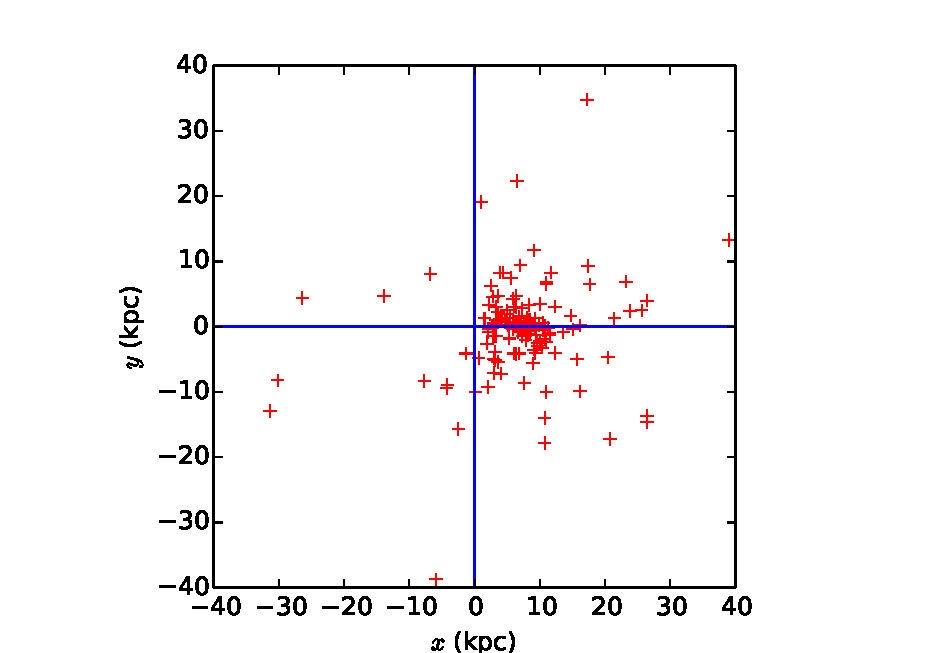
\includegraphics[width=\linewidth]{plan_xOy_GC.pdf}
				\end{minipage}\hfill
				\begin{minipage}{0.33\linewidth}
						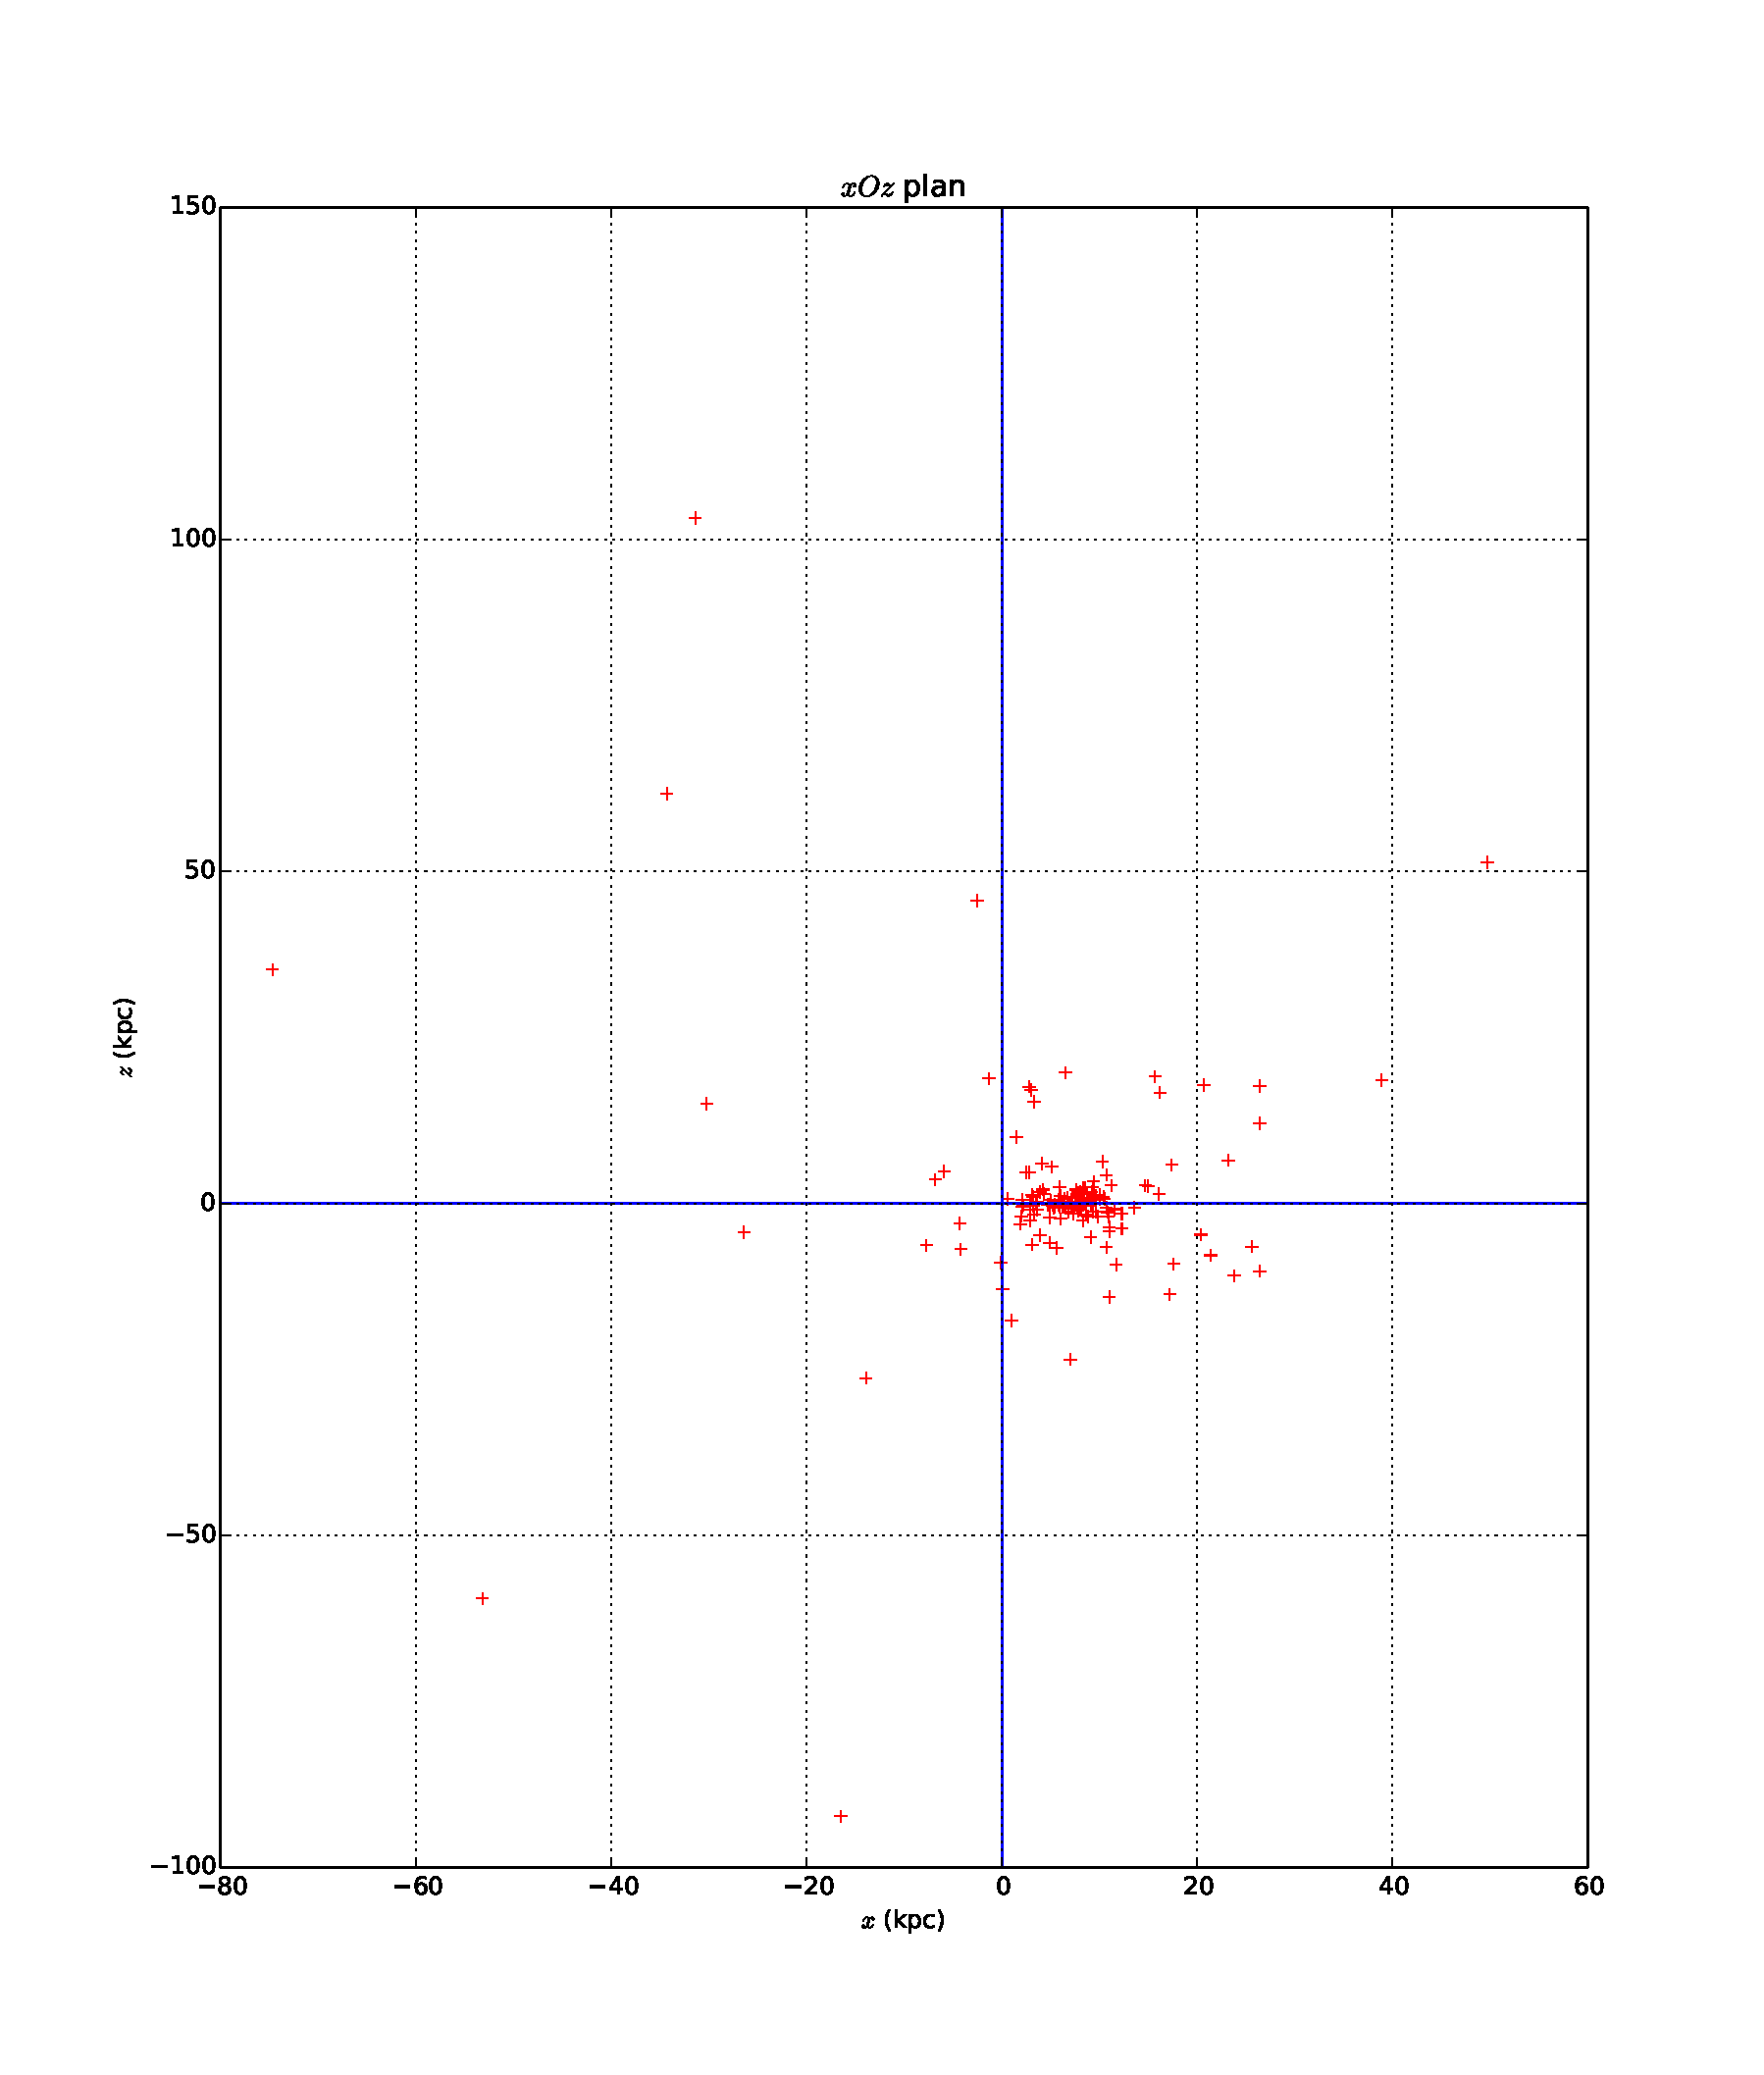
\includegraphics[width=\linewidth]{plan_xOz_GC.pdf}
				\end{minipage}\hfill
				\begin{minipage}{0.33\linewidth}
						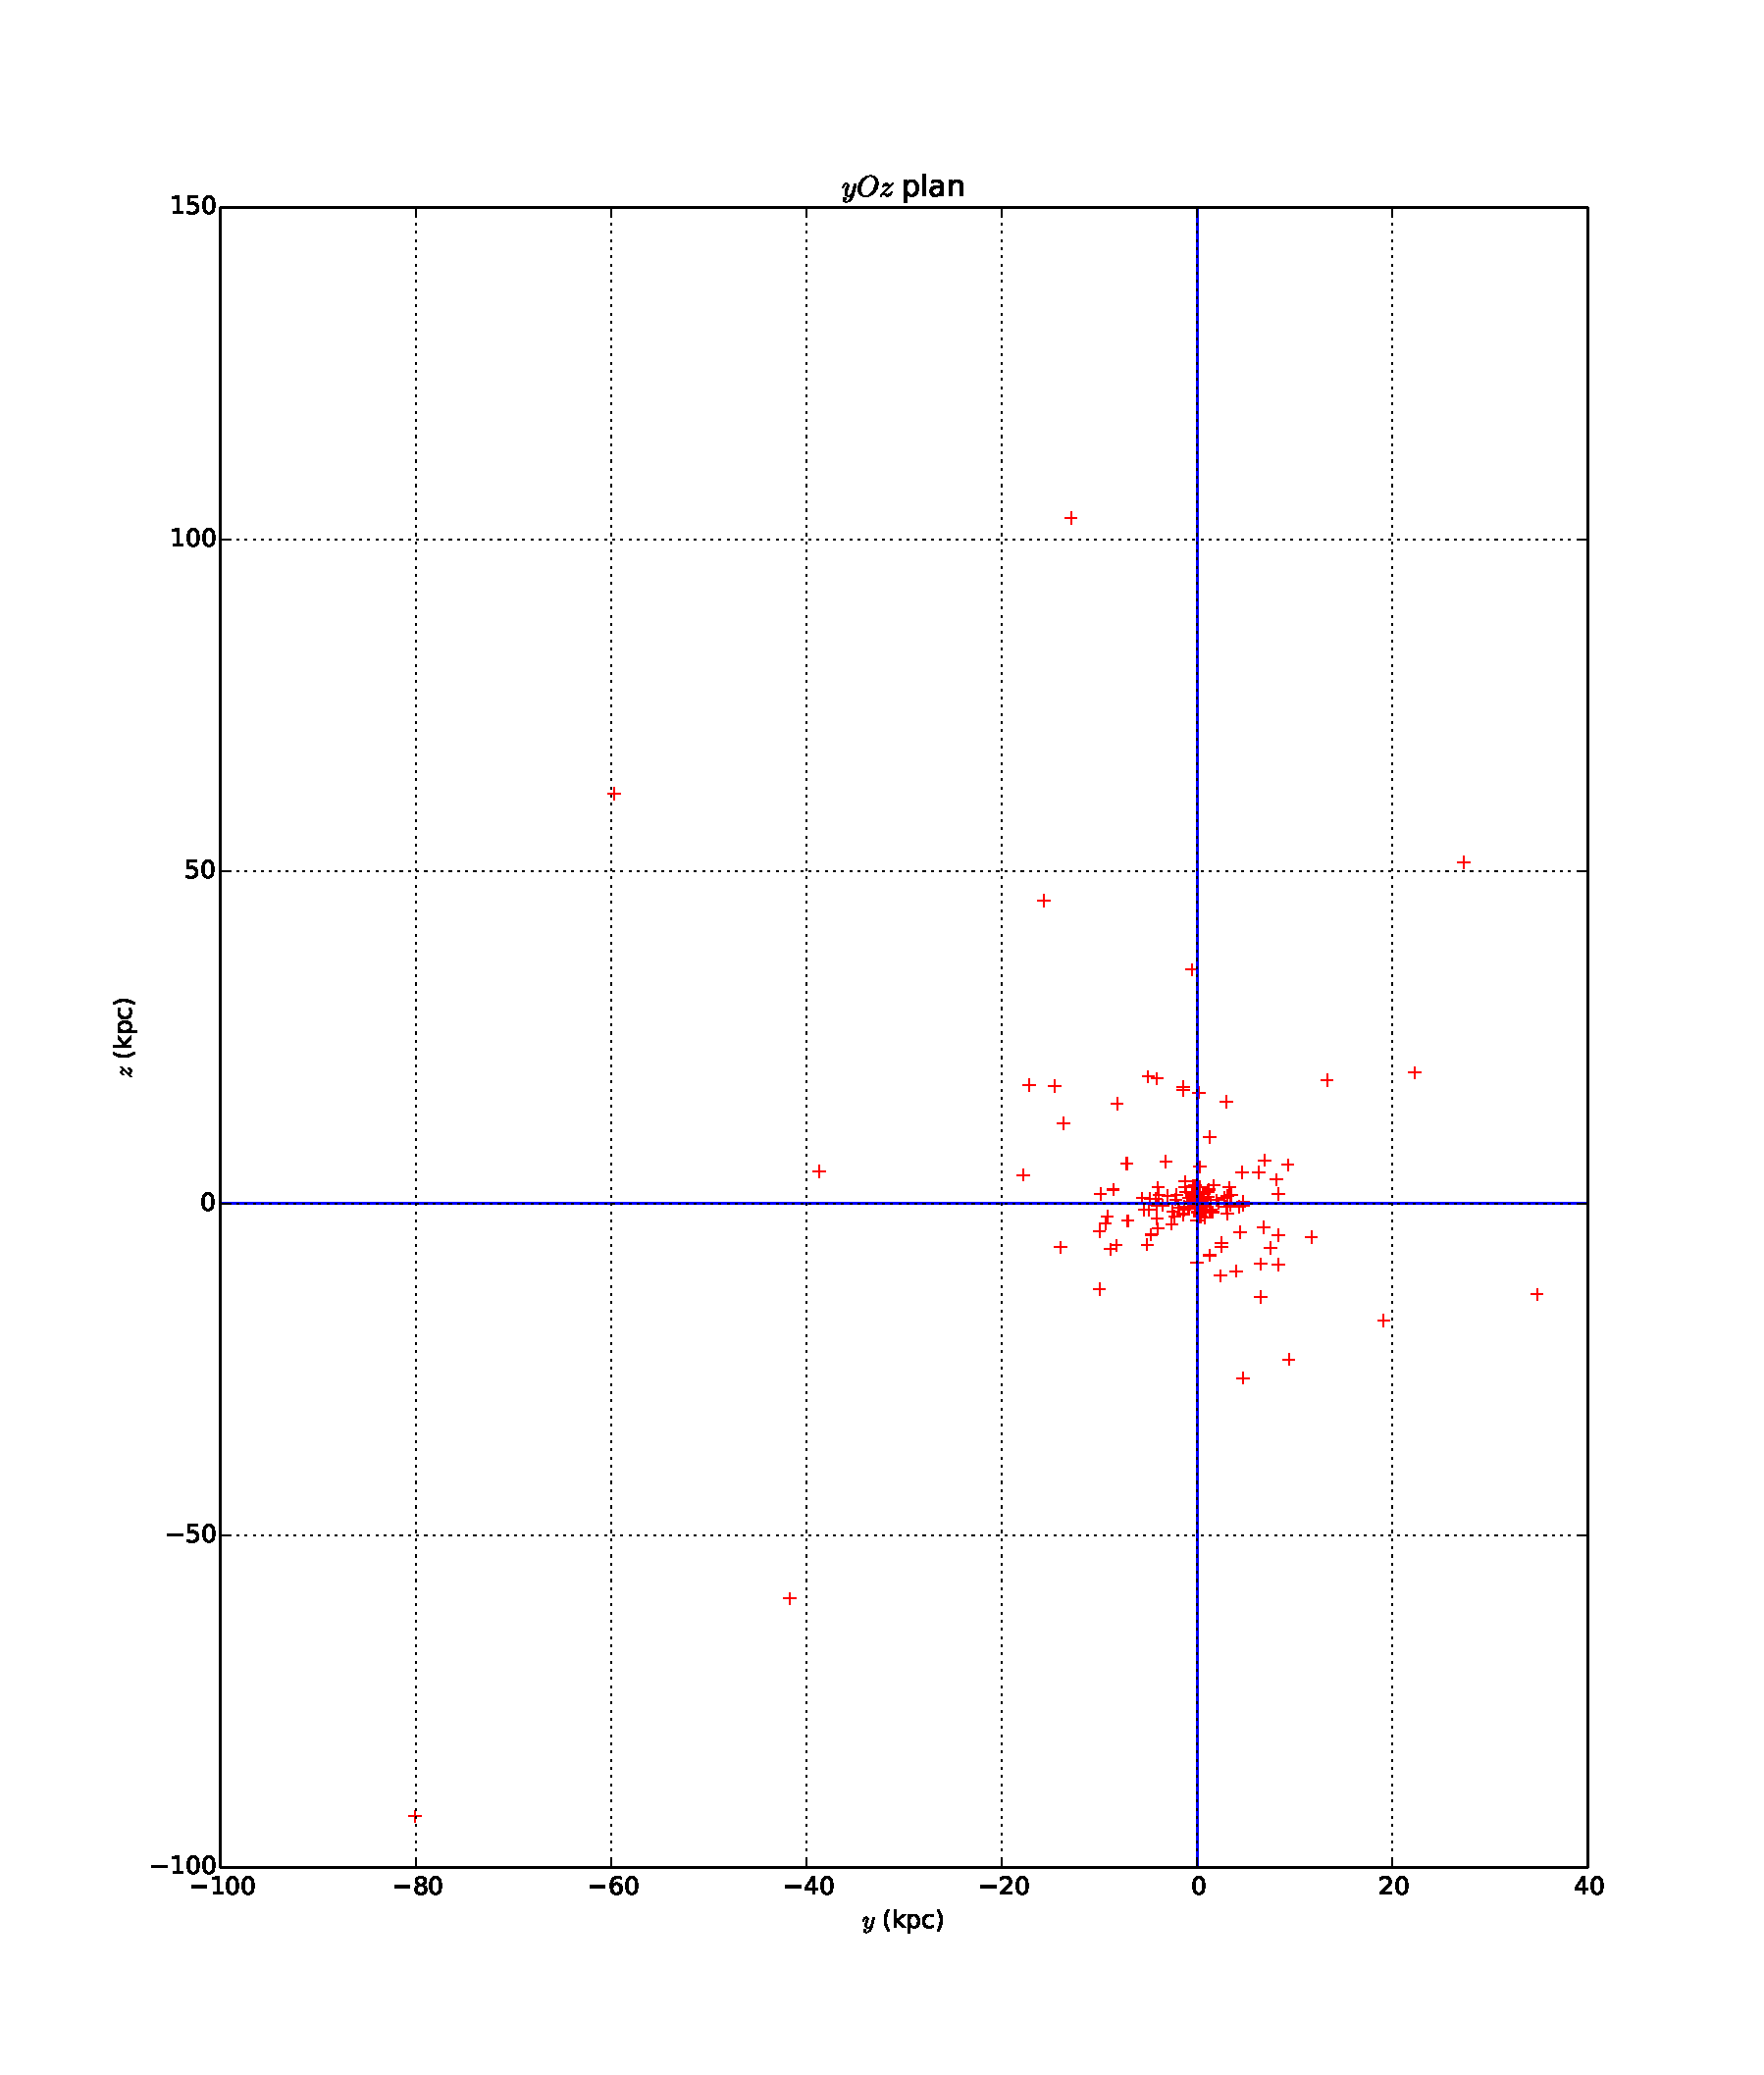
\includegraphics[width=\linewidth]{plan_yOz_GC.pdf}
				\end{minipage}
					\end{center}
				\caption{\label{Fig::Intro::repartition}Répartition des amas globulaires connus dans
				notre galaxie. Les graphiques utilisent le système de coordonnées galactiques (et donc centré sur le soleil).}
			\end{figure}


		\subsection{Profil de densité}

			L'étude des propriétés physiques des amas globulaires s'étale aujourd'hui sur plus d'un siècle d'observations et de
			modélisation. Une caractéristique commune aux amas est leur forme sphérique, l'ellipticité maximale observée étant de l'ordre
			de 10\% et s'explique par une faible rotation solide. Un consensus est maintenant établi sur le fait que leur profil de
			densité volumique de masse -- en abrégé densité et noté $\rho(r)$ -- est un excellent traceur de leur évolution. Les amas
			globulaires se répartissent en deux catégories (voir la figure~\ref{Fig::Intro::images}):
			\begin{itemize}

				\item 80\% des amas présentent une densité caractérisée par 2 régions: le cœur pour lequel la densité est quasiment
					constante ($\rho(r) \approx \mathrm{cte}$) et le halo dans lequel la densité évolue globalement comme une loi
					de puissance ($\rho(r) \propto r^{-\alpha}$): ils ont un profil de type cœur-halo (core-halo dans la
					littérature anglo-saxonne);

				\item la densité du cœur des 20\% restant est remplacée par une loi de puissance. Ils sont dits cœur effondré
					(core-collapsed).

			\end{itemize}

			La plupart des modèles d'amas globulaire sont issus de la sphère isotherme. Nous en
			aborderons certains au cours de ce document. Parmi ces modèles, un en particulier
			permet d'ajuster le profil de densité des amas globulaires durant une grande
			partie de leur évolution: le modèle de King
			(voir~\cite{1966AJ.....71...64K} et le chapitre~\ref{King::Chapitre}).

			\begin{figure}[h]
				\begin{center}
					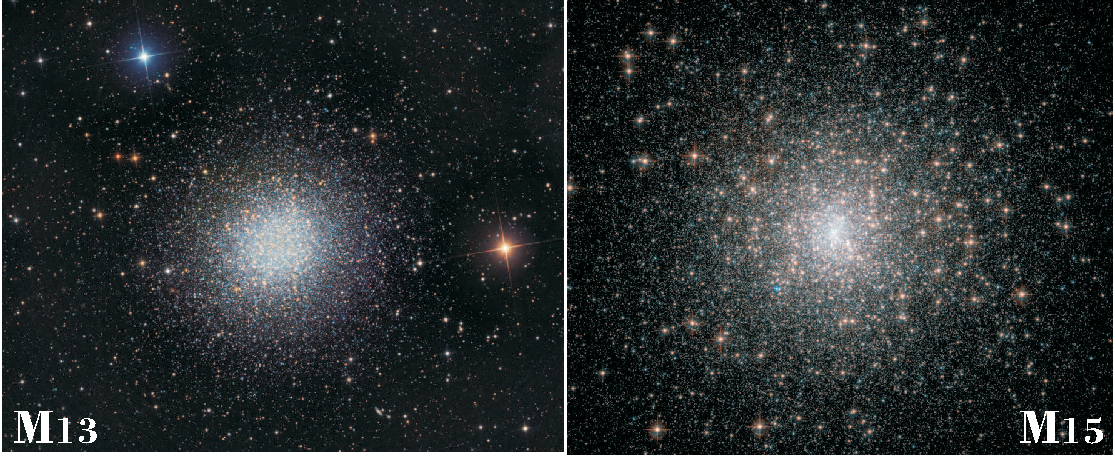
\includegraphics[width=\linewidth]{gc_photo}
				\end{center}
				\begin{minipage}{0.45\textwidth}
					\begin{center}
						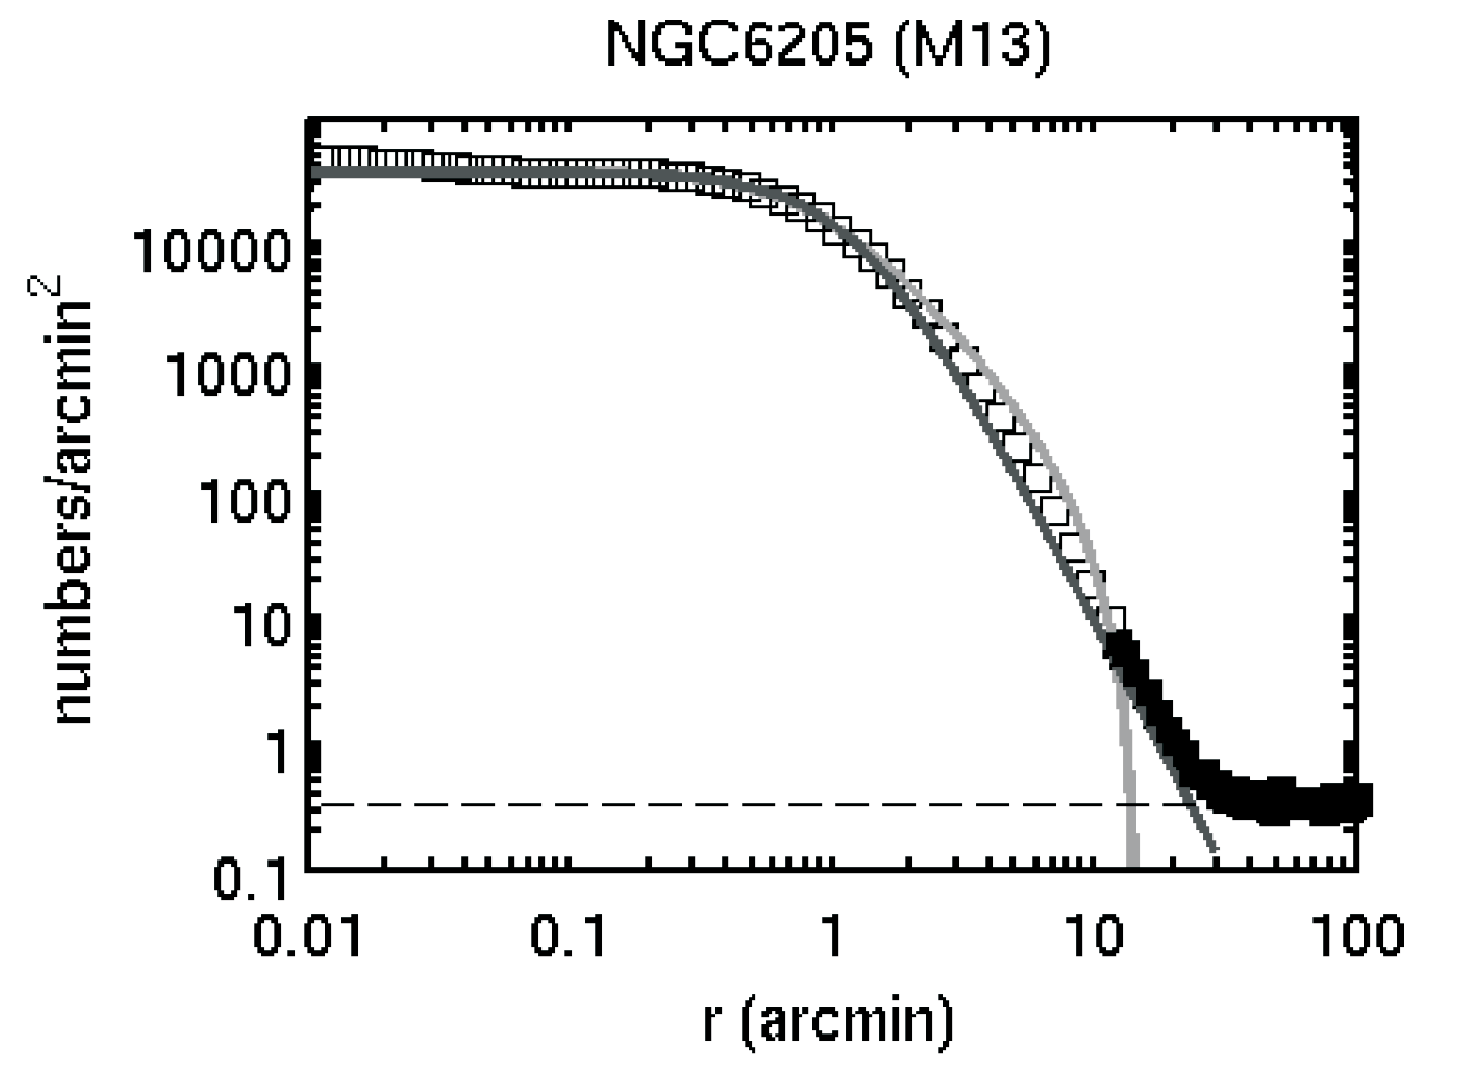
\includegraphics[width=\linewidth]{M13}
					\end{center}
				\end{minipage}\hfill
				\begin{minipage}{0.45\textwidth}
					\begin{center}
						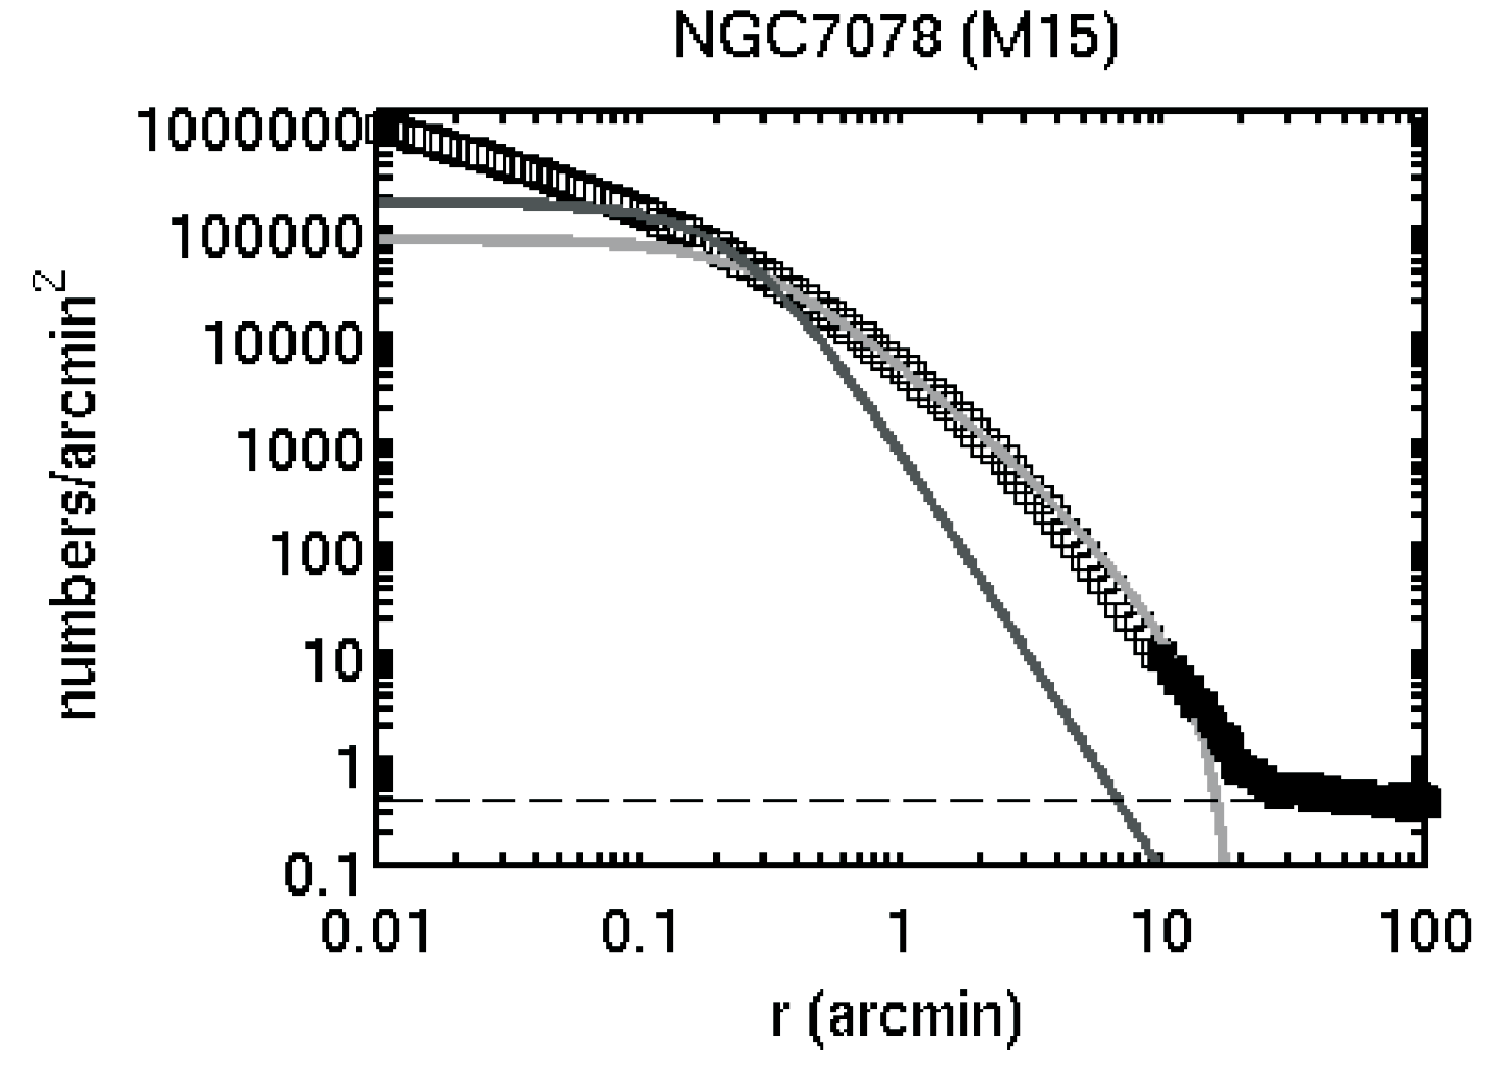
\includegraphics[width=\linewidth]{M15}
					\end{center}
				\end{minipage}
				\caption{\label{Fig::Intro::images}Deux amas globulaires
					caractéristiques et leurs comptages d'étoiles (tiré de~\cite{2010A&A...522A..71J}).
					M13 est un amas présentant une structure cœur-halo,
					M15 est un amas au cœur dit effondré}
			\end{figure}

		\subsection{Simulation numérique des amas globulaires}

			Dès les années 1960, des simulations numériques sont utilisées en plus de la théorie afin de modéliser l'évolution de ces
			objets. Plusieurs méthodes numériques ont été utilisées, les principales sont:
			\begin{itemize}

					\item les simulations Fokker-Planck permettent de
						simuler l'évolution d'un amas sphérique de plusieurs millions
						d'étoiles sur une grande période de temps en quelques
						jours de calcul. Même si ce type de simulation permet d'intégrer une
						certaine forme de dissipation dans l'évolution du système, une telle
						efficacité n'est possible qu'en faisant l'hypothèse que le système
						conserve ses propriétés sphériques et isotropes tout au long de son
						évolution;% L'algorithme utilisé est alors celui de Monte-Carlo;
						% Un algorithme de type Monte-Carlo est alors utilisé;

					% \item les simulations Monte-Carlo, elles permettent de
						% simuler l'évolution d'un amas de plusieurs millions
						% d'étoiles sur une grande période de temps en quelques
						% jours, en adaptant les propriétés globales des
						% orbites des étoiles au gré de leur évolution
						% numérique;

					\item les simulations $N$-corps utilisant une méthode de sommation directe modifient à chaque pas de
						temps les positions et vitesses des étoiles du modèle. Ces simulations sont beaucoup plus lentes mais
						laissent plus de liberté au système quant à son évolution.

					% \item les simulations $N$-corps utilisant un tree-code, méthode intermédiaire que nous utiliserons et qui sera
						% détaillée plus loin (voir le chapitre~\ref{Chap::Simu::Analysis}).

			\end{itemize}
			La figure~\ref{Fig::Intro::HeggieFigure}, issue de la présentation de D.~Heggie au trimestre Gravasco, montre les amas du
			catalogue de Harris tracés dans le plan (temps de relaxation)/(magnitude intégrée en bande V). Les droites parallèles
			indiquent le temps que durerait une simulation $N$-Corps (avec une sommation directe) ou Fokker-Planck d'un amas globulaire
			avec ces paramètres. Par exemple, une simulation $N$-Corps de l'évolution dynamique complète de M4 prendrait environ 300 ans
			tandis que son équivalent Fokker-Planck ne prendrait qu'une journée.

			\begin{figure}[h]
				\centering 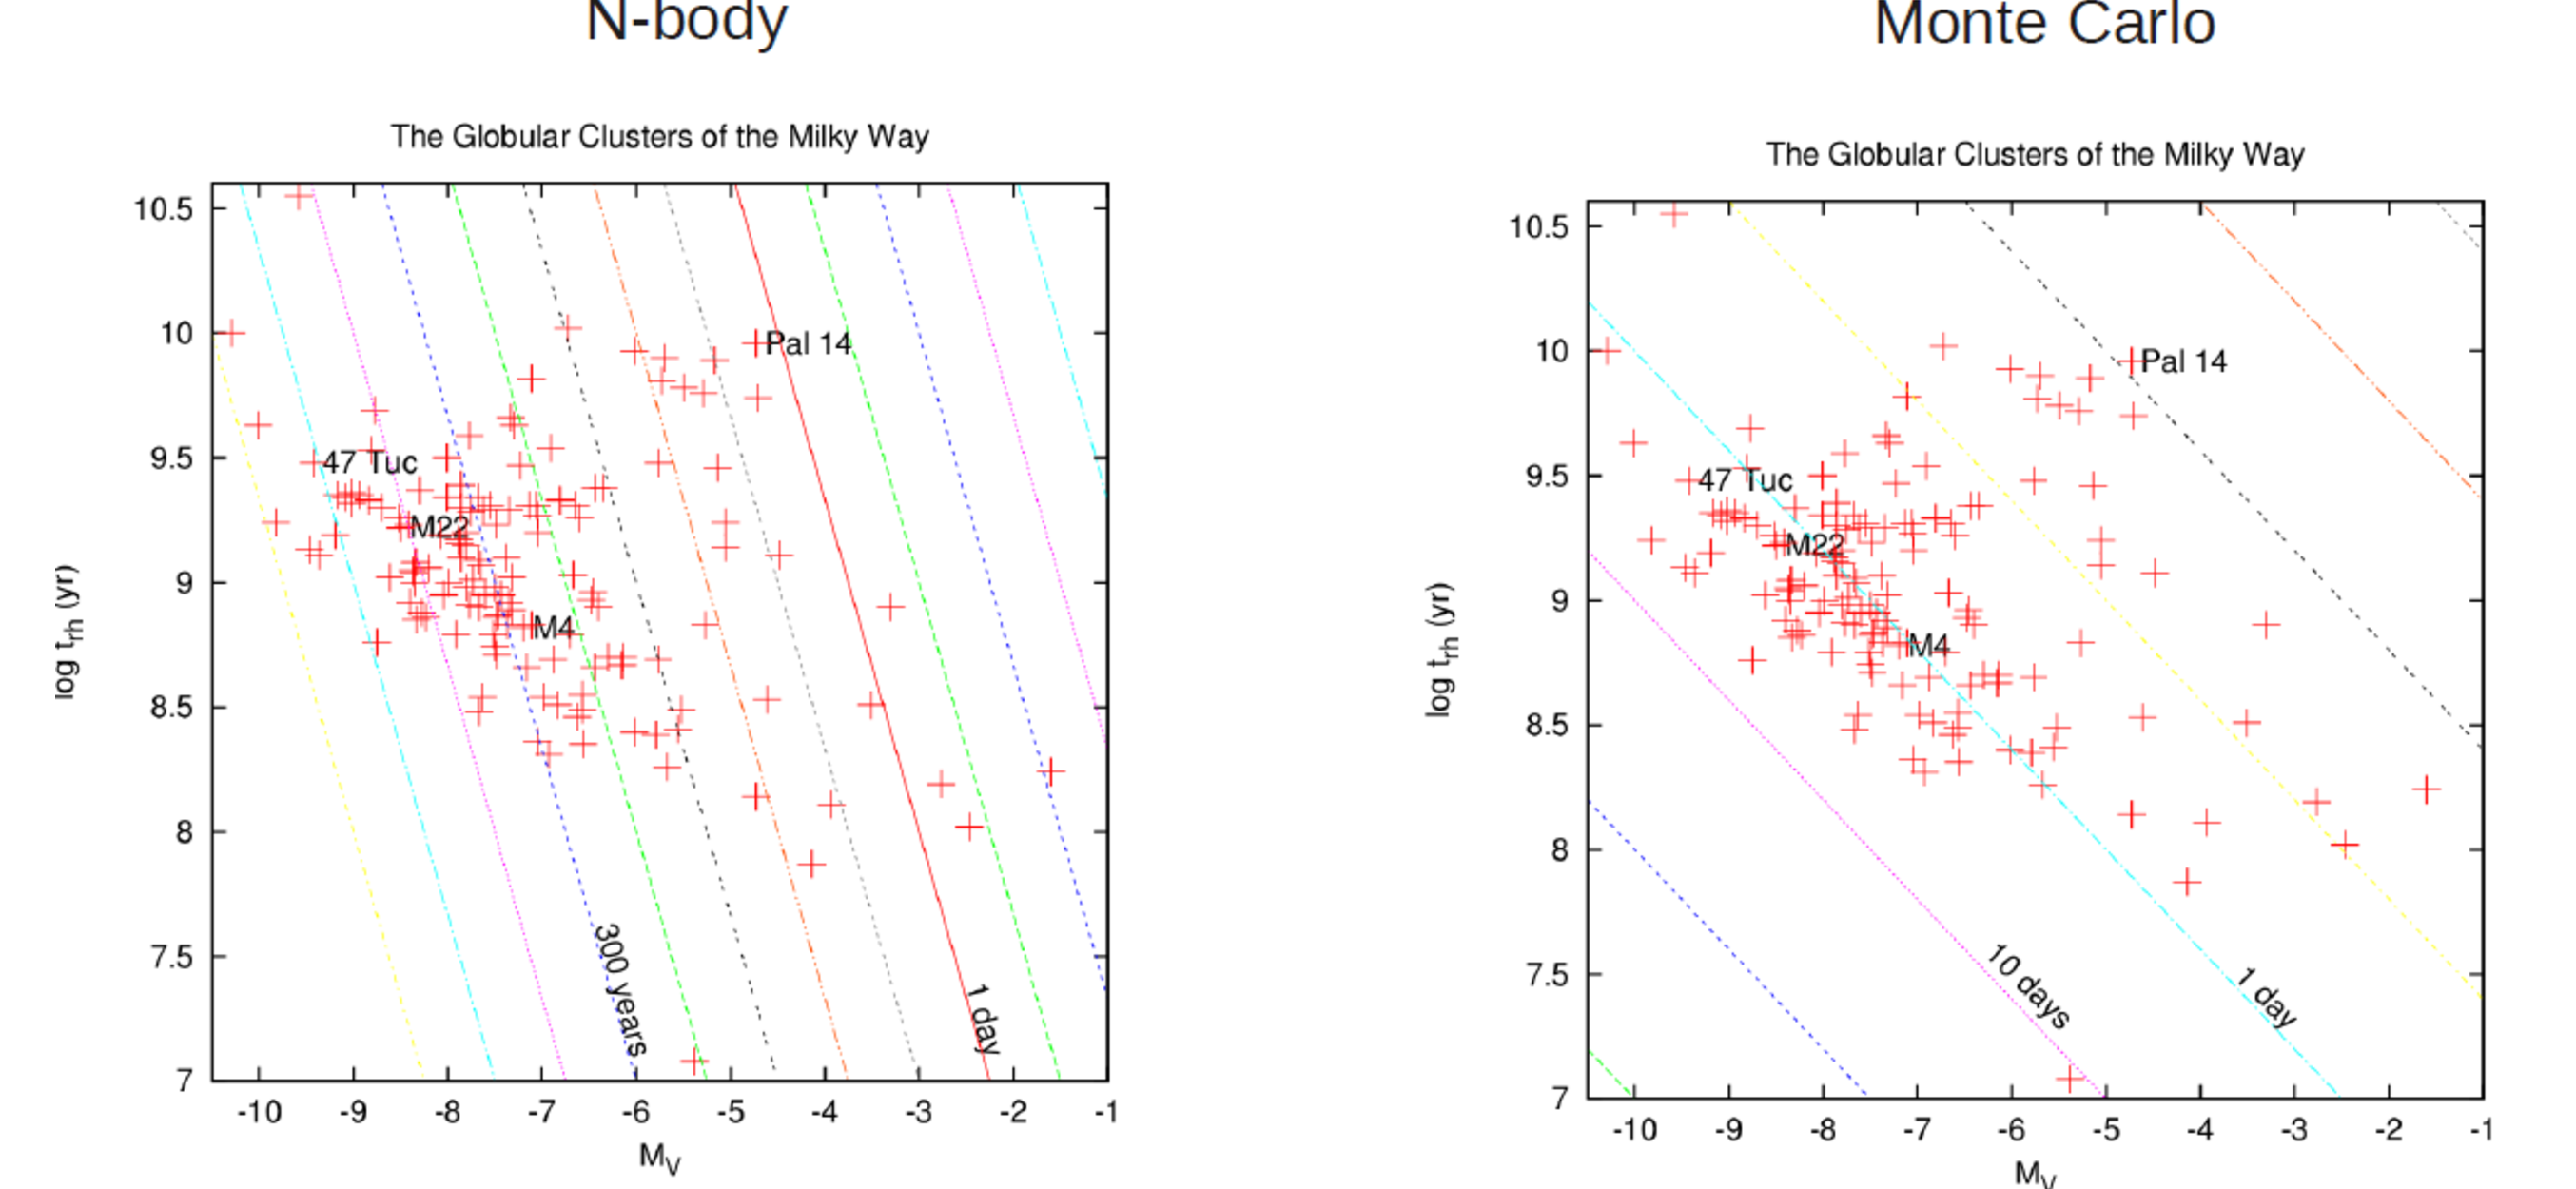
\includegraphics[width=\linewidth]{Heggie_figure.pdf}
				\caption{\label{Fig::Intro::HeggieFigure}Évolution du temps de
				calcul selon l'amas globulaire et du type de simulation.}
			\end{figure}

			Les simulations ont permis de prendre de l'avance sur les observations en
			confirmant certains phénomènes prévus par la théorie, notamment
			les oscillations gravothermales (voir~\cite{1996ApJ...471..796M}). Ce phénomène
			intervient après l'effondrement du cœur, une binaire serrée vient alors
			contrôler la dynamique du centre de l'amas. Sous l'effet d'interactions à 3
			corps, cette binaire est remplacée par une autre produisant un pic de
			densité. Ces pics se succèdent à un rythme dépendant des caractéristiques de
			l'amas.

			% Contrairement aux galaxies
			De façon générique,
			les amas globulaires ne semblent pas contenir
			en leur centre de trou noir massif. Par cet aspect, mais
			aussi par le fait qu'ils ne semblent pas contenir de grandes quantités de
			matière noire, ils se distinguent des galaxies.

		\subsection{Une première étude personnelle}

			Comme nous l'avons précisé plus haut, il est généralement admis que le
			profil de densité est un traceur de l'évolution des amas globulaires. Nous
			n'avons cependant pas trouvé d'étude exhaustive sur ce sujet et avons donc
			tenté de préciser ce lien.
			La principale caractéristique du profil de densité d'un amas globulaire est
			la pente de son halo. Celle-ci n'ayant pas fait l'objet d'une étude globale nous
			avons donc fabriqué notre propre catalogue à partir des données
			de~\cite{Trager-graphe} donnant le profil de brillance de surface en fonction de la taille angulaire
			de chaque amas.


			%Parallèlement, nous avons construit un catalogue
			%des temps de relaxation par collision de ces amas à partir du catalogue de
			%\textsc{Harris}~\cite{Harris}.

			%	Ce qui va nous intéresser ici, c'est de pouvoir lier à chaque étape d'évolution d'un amas, et donc à son âge,
			%	une pente.
				%Notre objectif est de trouver une relation entre l'âge d'un amas et la pente de son halo.
				%Nous avons parlé dans la section précédente du profil de densité
				%comme d'un marqueur de l'évolution des amas globulaires, nous allons
				%voir en quoi.
				%S'il est possible de trouver, à partir de ces profils, plusieurs
				%marqueur d'évolution, celui qui nous intéresse plus particulièrement
				%est la pente du halo. Pour vérifier que cette pente évolue bien avec
				%l'âge dynamique de l'objet, et comment, nous avons utilisé les
				%données du catalogue de \textsc{Harris}~\cite{Harris} qui nous a
				%permis d'obtenir l'âge d'une centaine d'amas
				%globulaire. Pour les profils de densité, nous
				%utilisons~\cite{Trager-graphe}.
				
				%Nous avons donc besoin d'une relation entre cette quantité et l'âge
				%de l'amas, si une telle relation existe.

				% Après avoir déprojeté les profils de brillance de surface
				% pour avoir la densité et donc obtenir la pente du halo, nous
				% l'avons tracé en fonction du temps de relaxation. Nous avons alors
				% ajusté la courbe ainsi obtenue par une droite d'équation $ \alpha =
				% \mathrm{pente} = a \log_{10}(T_c) + b$.

				% La première étape pour transformer les données
				% de~\cite{Trager-graphe} (récupérable ici~\cite{TragerTable}) d'une
				% brillance de surface de l'objet en fonction d'un rayon en seconde
				% d'arc en densité volumique de masse.

				%Le premier traitement à effectuer consiste donc à transformer
				%cette brillance de surface par arc seconde carrée en une densité
				%(~kilogramme par kilomètre au cube~).

				%Une définition de cette brillance de surface, telle qu'elle semble avoir été utilisée, peut-être trouvé dans~\cite{SBP}.
				%Comme indiqué dans ce texte, la brillance de surface va s'écrire :
				%\begin{align}
					%\mu_V = \mu_{\mathrm{ref}} - 2.5 \log_{10}\(\frac{f/\Omega}{f_{\mathrm{ref}}/\Omega_{\mathrm{ref}}}\)
					%\label{mu_V}
				%\end{align}
				%avec $\Omega$ l'angle solide, exprimé en seconde d'arc au carrée, sous lequel nous voyons l'objet.
			%	\begin{align}
			%		\mu_V = m_V - 2.5 \log_{10}\(\frac{(1\mathrm{"})^2}{\Omega}\)
			%		\label{mu-astuce}
			%	\end{align}
			%	avec $m_V$ la magnitude apparente de l'objet sur une seconde d'arc au carrée.

				La brillance de surface utilisée dans cet article est la suivante:
				\begin{align}
					\mu = -2.5 \log\(\frac{10^{-0.4 m_2} - 10^{-0.4 m_1}}{\pi \(r_2^2 - r_1^2\)}\)
					\label{Trager-eq}
				\end{align}
			%	où ils prendraient comme référence les points autour de celui considéré (~ou quelque chose comme ça~),
				$m_i$ étant la magnitude en un point de l'objet et $r_i$ le rayon en seconde d'arc pour ce point.

				La conversion de cette brillance surfacique en densité surfacique de masse est possible
				en connaissant le rapport masse-luminosité de ces amas. L'article~\cite{McL} ne donne cette
				quantité que pour 40 des 150 amas de notre galaxie.
				% Les rapports masse-luminosité dont nous avons besoin pour terminer
				% la conversion peuvent être trouvés dans~\cite{McL},
				% mais cette article ne contient que 40 des 140 amas de notre galaxie.
				Par contre, il est aisé de remarquer que ces rapports sont %en
				répartis dans un intervalle de faible amplitude
				% moyenne très peu différents de la valeur $2$
				avec une
				valeur minimum de $1.87$ pour NGC4147 et une valeur maximum de
				$2.66$ pour NGC6441. Pour simplifier, nous avons utilisé:
				%Dans la suite, nous prendrons donc:
				\begin{align}
					\Upsilon = \dfrac{M}{L} = 2
				\end{align}
				pour les 110 amas dont nous ne connaissons pas $\Upsilon$. %autres amas.
				%Les données de~\cite{Trager-graphe} nous ont donc permis d'obtenir
				Un algorithme de déprojection permet alors d'obtenir la densité $\rho(r)$ de chaque amas du catalogue de Harris.

				%\begin{enumerate}
					%\item $10^{-0.4 m_i}$ est proportionnel à un flux, % (~ou au rapport d'un flux par rapport à un flux de référence !?!~),
					%\item $r_i$ est le rayon de l'objet au point $i$ en seconde d'arc,
					%\item[$\Rightarrow$] nous avons donc bien notre flux par seconde d'arc au carrée.
				%\end{enumerate}
				%Pour pouvoir revenir aux quantités que nous cherchons, il va falloir calculer un peu :
				%\begin{align}
					%\mu = -2.5 \log\(\frac{10^{-0.4 m_2} - 10^{-0.4 m_1}}{\pi \(r_2^2 - r_1^2\)}\) &\equiv -2.5 \log\(\frac{F}{\pi \(r_2^2 - r_1^2\)}\) \text{avec $F$ le flux}\notag \\
					%\intertext{par rapport à toute la documentation que j'ai trouvé, le $\log$ correspond ici à $\log_{10}$ et non à $\ln$.}
					%\Rightarrow \frac{F}{\pi \(r_2^2 - r_1^2\)} &= 10^{-\mu/2.5} \label{F--mu} \\
					%\intertext{Grâce à~\cite{McL}, nous avons les rapports masse luminosité :}
					%\Upsilon &= \frac{M}{L} \label{M/L}\\
					%\intertext{or}
					%F &= \frac{L}{4\pi D^2} \label{def-F}\\
					%\intertext{avec $D$ la distance soleil--amas. D'où}
					%\frac{L}{4 \pi^2 \(r_2^2 - r_1^2\) D^2} &= \frac{M}{4 \pi^2 \Upsilon \(r_2^2 - r_1^2\) D^2} = 10^{-\mu/2.5} \notag \\
					%\intertext{en combinant~\ref{F--mu}, \ref{M/L} et~\ref{def-F}.}
					%\Rightarrow \frac{M}{4\pi \(r_2^2 - r_1^2\)} &= \pi\Upsilon D^2 10^{-\mu/2.5} \notag \\
					%\intertext{Mais $r_2^2 - r_1^2 \propto r_i^2$ doit être converti en mètre :}
					%%r_2^2 - r_1^2 &\propto r_i^2 \Rightarrow \(D \tan(r_i)\)^2 \varpropto \(D r_i\)^2 \notag \\
					%\Rightarrow \frac{M}{4\pi \(D \tan(r_i/3600)\)^2} &= \pi\Upsilon D^2 10^{-\mu/2.5} \label{M-don}
				%\end{align}
				%Normalement, nous avons maintenant une masse surfacique donnée par~\ref{M-don}.
			%	mais, étonnamment, la conversion de seconde d'arc à mètre n'a fait paraître
			%	aucun facteur numérique !!! J'ai peut-être un peu trop truandé.

				%Les rapports masse-luminosité peuvent être trouvés dans~\cite{McL}, mais cette article ne contient que 40 des 140 amas de notre galaxie.
			%	mais il n'y a qu'une quarantaine de rapport comparé à notre échantillon d'environ 140 amas.
				%Par contre, il est aisé de remarquer que ces rapports sont
				%en moyenne très peu différents de la valeur $\Upsilon = 2$ avec une valeur minimum de $1.87$ pour NGC 4147 et une valeur maximum de
				%$2.66$ pour NGC 6441. Dans la suite, nous prendrons donc $\Upsilon = 2$.
			%	Nous avons alors utilisé les données du catalogue pour redimensionner le tout, mais pour passer à la densité, nous avons besoin du rapport masse
			%	sur luminosité de l'amas qui peut-être trouvé dans~\cite{McL}.
			%	Cet article ne donne qu'une quarantaine d'amas sur les 150 de notre galaxie, mais les valeurs de ces rapports étant compris entre $1.87$ pour NGC 4147
			%	(~et quelques autres~) et $2.66$ pour NGC 6441, et tournant surtout autour de $2$, nous pouvons supposer que ces rapports sont les mêmes pour chaque amas et
			%	valent $\Upsilon = \frac{M}{L} = 2$.
			%	Selon~\cite{Trager-graphe}, nous avons donc :
			%	\begin{align}
			%		\mu_V &\propto \text{Flux par $m^{-2}$} = \frac{L}{4\pi D^2} \\
			%		\intertext{or}
			%		L &= \frac{M}{\Upsilon} \notag \\
			%		\intertext{donc}
			%		\mu_V &= \frac{M}{4\pi D^2 \Upsilon} \notag \\
			%		M &= \Upsilon \mu_V 4\pi D^2
			%	\end{align}
			%	avec $D$ la distance entre nous et l'amas. Nous pouvons supposer que cette distance est la même quelque soit l'étoile considéré dans l'amas
			%	(~$D_{min} = 3000\mathrm{pc} \gg R_{amas} \approx 10\mathrm{pc}$~).

			%	Du fait des rapports masse-luminosité manquant, notre échantillon d'une quarantaine d'amas est passé à seulement 12 amas.

				Afin de déterminer la pente du halo, nous
				normalisons cette densité par la densité du cœur, puis mesurons la
				pente dans l'intervalle: %la région vérifiant:
				\begin{align*}
					10^{-4} \leq \dfrac{\rho(r)}{\rho(0)} \leq 0.1.
				\end{align*}
				Nous avons alors construit un catalogue des temps de relaxation par
				collisions et des temps dynamiques de ces amas en utilisant d'une part le catalogue de
				\cite{Harris} et d'autre part en intégrant le profil de densité obtenu
				pour chaque amas.
				Nous obtenons alors les graphiques~\ref{Pente-lin_dim} et~\ref{Pente-Td-lin}. L'ajustement a été effectué à l'aide
				d'une méthode de moindre carré, donnant une valeur de la pente de chaque droite de $-1.31\pm0.44$ pour la
				figure~\ref{Pente-Td-lin} et $-1.23\pm0.46$ pour la figure~\ref{Pente-lin_dim}. La valeur numérique de cette pente
				n'est pas fondamentale, une tendance est cependant bien présente: la pente diminue lorsque le temps dynamique ou le
				temps de collision augmente.

				%Le calcul de pente a été refait en utilisant : les données de
				%l'article~\cite{TragerTable}, le traitement décrit ci-dessus, et en
				%ajustant une droite pour des densités comprises entre $10^{-4}$ et
				%0,1. Nous obtenons alors le graphique~\ref{Pente-lin_dim},
				%l'ajustement utilisant la fonction $f(T_c) = a \log(T_c) + b$ (~les
				%coefficients ont été donnés dans la
				%table~\ref{pente-lin-coeff_dim}~). Nous avons donc maintenant une
				%relation linéaire entre l'âge de l'amas et la pente du halo.

				\begin{figure}[h!]
			%		\centering \includegraphics[scale=0.9]{../Amas/Graphe_Rapport/pente-Tc.pdf}
					\centering 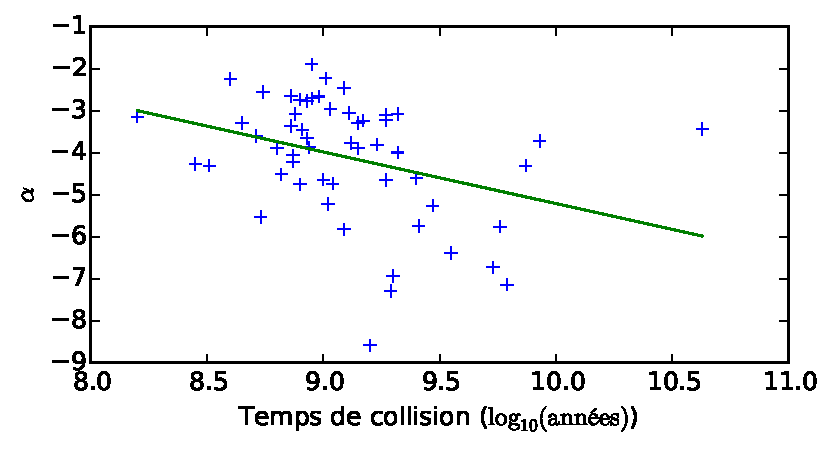
\includegraphics[scale=1.0]{graphe/pente_tc.pdf}
					\caption{Évolution des pentes pour différents âges collisionnels}
					\label{Pente-lin_dim}
				\end{figure}
				%\begin{table}[hbt!]
					%\begin{center}
						%\begin{tabular}{|c|c|}%c|}
							%\hline
							%Coefficient & Valeur \\ %& Erreur \\
							%\hline
							%\hline
							%$a$       &         $-2.3341$   \\ %&    $\pm 0.2075$      (~$32.34\%$~) \\
							%\hline
							%$b$       &         $16.913$   \\  %&    $\pm 1.638$       (~$199.5\%$~) \\
							%\hline
						%\end{tabular}
					%\end{center}
					%\caption{Valeurs des coefficients donnée par l'ajustement pour les pentes pour le temps de croisement}
					%\label{pente-lin-coeff_dim}
				%\end{table}

				%Nous avons également utilisé le catalogue de \textsc{Harris} pour obtenir le lien entre la pente du halo et le temps dynamique
				%grâce à l'équation~\ref{Td:sig}. Nous obtenons alors le graphique~\ref{Pente-Td-lin}.
				\begin{figure}[h!]
			%		\centering \includegraphics[scale=0.9]{../Amas/Graphe_Rapport/pente-Td.pdf}
					\centering 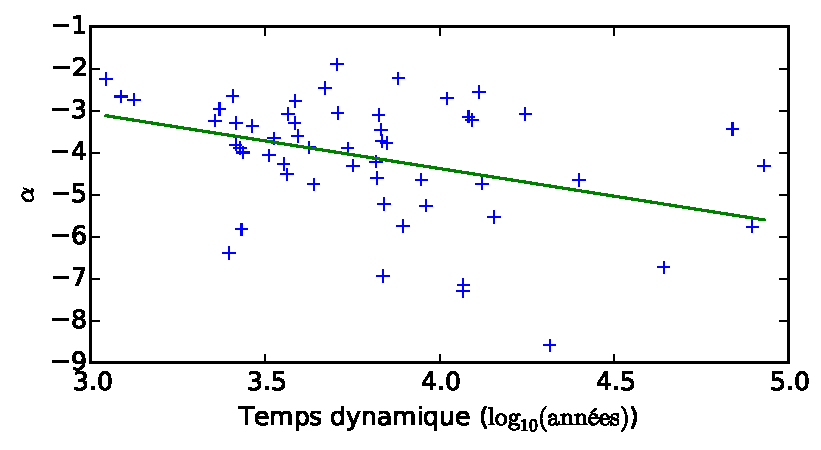
\includegraphics[scale=1.0]{graphe/pente_td.pdf}
					\caption{Évolution des pentes pour différents âges dynamiques}
					\label{Pente-Td-lin}
				\end{figure}
				%\begin{table}[hbt!]
					%\begin{center}
						%\begin{tabular}{|c|c|}%c|}
							%\hline
							%Coefficient & Valeur \\ %& Erreur \\
							%\hline
							%\hline
							%$a$       &        $-1.6567$   \\ %&   $\pm 0.6523$      (~$278.9\%$~) \\
							%\hline
							%$b$       &        $1.8927$     \\ %&   $\pm 2.825$       (~$88.57\%$~) \\
							%\hline
						%\end{tabular}
					%\end{center}
					%\caption{Valeurs des coefficients donnée par l'ajustement pour les pentes pour le temps dynamique}
					%\label{pente-Td-lin-coeff}
				%\end{table}

				%Sur la figure~\ref{Pente-lin_dim}, nous pouvons noter la présence de 2 points avec des pentes inférieures à $-10$. Ces points correspondent aux amas NGC 5024 et NGC 5139
				%(~leurs densités sont donnée en annexe, page~\pageref{Graphe-bofbof}~) pour lesquelles la détermination des pentes n'a pas été très concluante.
				%\FloatBarrier

		%\subsection{Préliminaire}
%	Ce qui va nous intéresser ici, c'est de pouvoir lier à chaque étape d'évolution d'un amas, et donc à son âge,
%	une pente.
	Notre objectif est de trouver une relation entre l'âge d'un amas et la pente de son halo.
	%Nous avons donc besoin d'une relation entre cette quantité et l'âge de l'amas, si une telle relation existe.
	Nous avons alors utilisé le temps de relaxation donné dans le catalogue de \textsc{Harris}~\cite{Harris}.
	Pour obtenir les pentes des amas, nous avons utilisé les relevés observationnels~\cite{Trager-graphe}. % (~les données ainsi obtenues et utilisées sont dans la table~\ref{pente-Tc:BSP}~).
	Nous avons commencé par calculer les pentes directement sur les courbes avec un double décimètre, n'ayant alors pas pu obtenir les données correspondant aux graphiques.
	Après avoir tracé la pente mesurée en fonction du temps de relaxation à 2 corps, nous avons ajusté la
	courbe ainsi obtenue par une droite d'équation $ \alpha = \mathrm{pente} = a \log_{10}(T_c) + b$ (~graphe~\ref{Pente-lin}~).
	\begin{figure}[hbt!]
		\centering \includegraphics[scale=0.9]{graphe/Pente-Tc.pdf}
		\caption{Évolution des pentes pour différents âges}
		\label{Pente-lin}
	\end{figure}
%	\begin{table}[hbt!]
%		\begin{center}
%			\begin{tabular}{|c|c|c|}
%				\hline
%				Coefficient & Valeur & Erreur \\
%				\hline
%				\hline
%				$a$       &        $-1.19506$   &   $\pm 0.1576$ (~$13.19\%$~) \\
%				\hline
%				$b$       &        $2.52082$     &   $\pm 1.213$   (~$48.11\%$~) \\
%				\hline
%			\end{tabular}
%		\end{center}
%		\caption{Valeur des coefficients donnée par l'ajustement pour les pentes}
%		\label{pente-lin-coeff}
%	\end{table}

	Cette approche indiquant clairement une relation linéaire entre ces deux paramètres, nous avons décidé d'entreprendre une démarche plus globale et automatique.
	Pour commencer, nous avons donc récupéré les données auprès des auteurs de l'article sur~\cite{TragerTable}. Nous nous sommes alors confronté au problème des unités.

\subsection{Retraitement}
	Le graphique~\ref{Pente-lin} a été obtenu en utilisant~\cite{Trager-graphe} avec ses unités. % (~les données permettant de retracer, nous les avons finalement trouvé,
%	les graphiques de cet article sont données dans~\cite{TragerTable}~).
	La pente donnée ici n'est donc pas la pente de la densité, mais de la brillance de surface de l'objet en fonction d'un rayon en seconde d'arc.
	Le premier traitement à effectuer consiste donc à transformer cette brillance de surface par arc seconde carrée en une densité (~kilogramme par kilomètre au cube~).

	Une définition de cette brillance de surface, telle qu'elle semble avoir été utilisée, peut-être trouvé dans~\cite{SBP}.
	Comme indiqué dans ce texte, la brillance de surface va s'écrire :
	\begin{align}
		\mu_V = \mu_{\mathrm{ref}} - 2.5 \log_{10}\(\frac{f/\Omega}{f_{\mathrm{ref}}/\Omega_{\mathrm{ref}}}\)
		\label{mu_V}
	\end{align}
	avec $\Omega$ l'angle solide, exprimé en seconde d'arc au carrée, sous lequel nous voyons l'objet.
%	\begin{align}
%		\mu_V = m_V - 2.5 \log_{10}\(\frac{(1\mathrm{"})^2}{\Omega}\)
%		\label{mu-astuce}
%	\end{align}
%	avec $m_V$ la magnitude apparente de l'objet sur une seconde d'arc au carrée.

	Cette définition rappelle celle de~\cite{Trager-graphe}, section~3.2.3 :
	\begin{align}
		\mu = -2.5 \log\(\frac{10^{-0.4 m_2} - 10^{-0.4 m_1}}{\pi \(r_2^2 - r_1^2\)}\)
		\label{Trager-eq}
	\end{align}
%	où ils prendraient comme référence les points autour de celui considéré (~ou quelque chose comme ça~),
	$m_i$ étant la magnitude en un point de l'objet et $r_i$ le rayon en seconde d'arc pour ce point.
	Par conséquent, les unités de $\mu$ sont un flux par arc seconde carrée en échelle logarithmique :
	\begin{enumerate}
		\item $10^{-0.4 m_i}$ est proportionnel à un flux, % (~ou au rapport d'un flux par rapport à un flux de référence !?!~),
		\item $r_i$ est le rayon de l'objet au point $i$ en seconde d'arc,
		\item[$\Rightarrow$] nous avons donc bien notre flux par seconde d'arc au carrée.
	\end{enumerate}
	Pour pouvoir revenir aux quantités que nous cherchons, il va falloir calculer un peu :
	\begin{align}
		\mu = -2.5 \log\(\frac{10^{-0.4 m_2} - 10^{-0.4 m_1}}{\pi \(r_2^2 - r_1^2\)}\) &\equiv -2.5 \log\(\frac{F}{\pi \(r_2^2 - r_1^2\)}\) \text{avec $F$ le flux}\notag \\
		\intertext{par rapport à toute la documentation que j'ai trouvé, le $\log$ correspond ici à $\log_{10}$ et non à $\ln$.}
		\Rightarrow \frac{F}{\pi \(r_2^2 - r_1^2\)} &= 10^{-\mu/2.5} \label{F--mu} \\
		\intertext{Grâce à~\cite{McL}, nous avons les rapports masse luminosité :}
		\Upsilon &= \frac{M}{L} \label{M/L}\\
		\intertext{or}
		F &= \frac{L}{4\pi D^2} \label{def-F}\\
		\intertext{avec $D$ la distance soleil--amas. D'où}
		\frac{L}{4 \pi^2 \(r_2^2 - r_1^2\) D^2} &= \frac{M}{4 \pi^2 \Upsilon \(r_2^2 - r_1^2\) D^2} = 10^{-\mu/2.5} \notag \\
		\intertext{en combinant~\ref{F--mu}, \ref{M/L} et~\ref{def-F}.}
		\Rightarrow \frac{M}{4\pi \(r_2^2 - r_1^2\)} &= \pi\Upsilon D^2 10^{-\mu/2.5} \notag \\
		\intertext{Mais $r_2^2 - r_1^2 \propto r_i^2$ doit être converti en mètre :}
		%r_2^2 - r_1^2 &\propto r_i^2 \Rightarrow \(D \tan(r_i)\)^2 \varpropto \(D r_i\)^2 \notag \\
		\Rightarrow \frac{M}{4\pi \(D \tan(r_i/3600)\)^2} &= \pi\Upsilon D^2 10^{-\mu/2.5} \label{M-don}
	\end{align}
	Normalement, nous avons maintenant une masse surfacique donnée par~\ref{M-don}.
%	mais, étonnamment, la conversion de seconde d'arc à mètre n'a fait paraître
%	aucun facteur numérique !!! J'ai peut-être un peu trop truandé.

	Les rapports masse-luminosité peuvent être trouvés dans~\cite{McL}, mais cette article ne contient que 40 des 140 amas de notre galaxie.
%	mais il n'y a qu'une quarantaine de rapport comparé à notre échantillon d'environ 140 amas.
	Par contre, il est aisé de remarquer que ces rapports sont
	en moyenne très peu différents de la valeur $\Upsilon = 2$ avec une valeur minimum de $1.87$ pour NGC 4147 et une valeur maximum de
	$2.66$ pour NGC 6441. Dans la suite, nous prendrons donc $\Upsilon = 2$.
%	Nous avons alors utilisé les données du catalogue pour redimensionner le tout, mais pour passer à la densité, nous avons besoin du rapport masse
%	sur luminosité de l'amas qui peut-être trouvé dans~\cite{McL}.
%	Cet article ne donne qu'une quarantaine d'amas sur les 150 de notre galaxie, mais les valeurs de ces rapports étant compris entre $1.87$ pour NGC 4147
%	(~et quelques autres~) et $2.66$ pour NGC 6441, et tournant surtout autour de $2$, nous pouvons supposer que ces rapports sont les mêmes pour chaque amas et
%	valent $\Upsilon = \frac{M}{L} = 2$.
%	Selon~\cite{Trager-graphe}, nous avons donc :
%	\begin{align}
%		\mu_V &\propto \text{Flux par $m^{-2}$} = \frac{L}{4\pi D^2} \\
%		\intertext{or}
%		L &= \frac{M}{\Upsilon} \notag \\
%		\intertext{donc}
%		\mu_V &= \frac{M}{4\pi D^2 \Upsilon} \notag \\
%		M &= \Upsilon \mu_V 4\pi D^2
%	\end{align}
%	avec $D$ la distance entre nous et l'amas. Nous pouvons supposer que cette distance est la même quelque soit l'étoile considéré dans l'amas
%	(~$D_{min} = 3000\mathrm{pc} \gg R_{amas} \approx 10\mathrm{pc}$~).

%	Du fait des rapports masse-luminosité manquant, notre échantillon d'une quarantaine d'amas est passé à seulement 12 amas.

\subsection{Résultat}
	Le calcul de pente a été refait en utilisant : les données de l'article~\cite{TragerTable}, le traitement décrit ci-dessus, et le critère donné dans la section~\ref{pente-critére}.
	Nous obtenons alors le graphique~\ref{Pente-lin_dim}, l'ajustement utilisant la fonction
	$f(T_c) = a \log(T_c) + b$ (~les coefficients ont été donnés dans la table~\ref{pente-lin-coeff_dim}~).
	Nous avons donc maintenant une relation linéaire entre l'âge de l'amas et la pente du halo.

	\begin{figure}[hbt!]
%		\centering \includegraphics[scale=0.9]{../Amas/Graphe_Rapport/pente-Tc.pdf}
		\centering \includegraphics[scale=0.9]{graphe/pente-Tc.pdf}
		\caption{Évolution des pentes pour différents âges}
		\label{Pente-lin_dim}
	\end{figure}
	\begin{table}[hbt!]
		\begin{center}
			\begin{tabular}{|c|c|}%c|}
				\hline
				Coefficient & Valeur \\ %& Erreur \\
				\hline
				\hline
				$a$       &         $-2.3341$   \\ %&    $\pm 0.2075$      (~$32.34\%$~) \\
				\hline
				$b$       &         $16.913$   \\  %&    $\pm 1.638$       (~$199.5\%$~) \\
				\hline
			\end{tabular}
		\end{center}
		\caption{Valeurs des coefficients donnée par l'ajustement pour les pentes pour le temps de croisement}
		\label{pente-lin-coeff_dim}
	\end{table}

	Nous avons également utilisé le catalogue de \textsc{Harris} pour obtenir le lien entre la pente du halo et le temps dynamique
	grâce à l'équation~\ref{Td:sig}. Nous obtenons alors le graphique~\ref{Pente-Td-lin}.
	\begin{figure}[hbt!]
%		\centering \includegraphics[scale=0.9]{../Amas/Graphe_Rapport/pente-Td.pdf}
		\centering \includegraphics[scale=0.9]{graphe/pente-Td.pdf}
		\caption{Évolution des pentes pour différents âges dynamiques}
		\label{Pente-Td-lin}
	\end{figure}
	\begin{table}[hbt!]
		\begin{center}
			\begin{tabular}{|c|c|}%c|}
				\hline
				Coefficient & Valeur \\ %& Erreur \\
				\hline
				\hline
				$a$       &        $-1.6567$   \\ %&   $\pm 0.6523$      (~$278.9\%$~) \\
				\hline
				$b$       &        $1.8927$     \\ %&   $\pm 2.825$       (~$88.57\%$~) \\
				\hline
			\end{tabular}
		\end{center}
		\caption{Valeurs des coefficients donnée par l'ajustement pour les pentes pour le temps dynamique}
		\label{pente-Td-lin-coeff}
	\end{table}

	Sur la figure~\ref{Pente-lin_dim}, nous pouvons noter la présence de 2 points avec des pentes inférieures à $-10$. Ces points correspondent aux amas NGC 5024 et NGC 5139
	(~leurs densités sont donnée en annexe, page~\pageref{Graphe-bofbof}~) pour lesquelles la détermination des pentes n'a pas été très concluante.
	\FloatBarrier



	%\section{Interprétation}

%Nous avons maintenant une équation liant la valeur de la pente au temps de relaxation : $ \mathrm{pente} = \alpha = d * \log_{10}(T_c) + e $ (~coefficients table~\ref{pente-lin-coeff_dim}~)
%et une autre liant la pente à $W_0$ : $ \alpha = a e^{ b W_0 } + c $.
%En combinant ces deux équations, nous pouvons obtenir une relation entre le temps de
%relaxation et $W_0$ :
%\begin{align}
	%\mathrm{pente} &= d \log_{10}(T_c) + e = a e^{b W_0} + c \notag \\
	%\Rightarrow W_0 &= \frac{1}{b} \ln\( \frac{d \log_{10}(T_c) + e - c}{a} \) \label{Tc:W0->fct}
%\end{align}
%avec :
%\begin{table}[h!]
	%\begin{center}
		%\begin{tabular}{|c|r|}
			%\hline
			%Coefficient	&	Valeur \\
			%\hline
			%\hline
			%$a$		&	$ -10.0698 $ \\
				%\hline
			%$b$		&	$ 0.220152 $ \\
			%\hline
			%$c$		&	$ -1.53409 $ \\
			%\hline
			%$d$		&	$ -2.3341 $ \\
			%\hline
			%$e$		&	$ 16.913 $ \\
			%\hline
		%\end{tabular}
	%\end{center}
%\end{table}

%Le comportement que nous avions observé en étudiant le modèle de \textsc{King}, à savoir une évolution de la pente avec $W_0$, se retrouve avec l'âge de notre amas. Ce qui nous a permis de relier
%l'âge et $W_0$.
%Il nous reste à interpreter ces résultats, ce que nous allons faire dans la section suivante.
		%Nous avons maintenant une équation liant la valeur de la pente au temps de relaxation : $ \mathrm{pente} = \alpha = d * \log_{10}(T_c) + e $ (~coefficients table~\ref{pente-lin-coeff_dim}~)
et une autre liant la pente à $W_0$ : $ \alpha = a e^{ b W_0 } + c $.
En combinant ces deux équations, nous pouvons obtenir une relation entre le temps de
relaxation et $W_0$ :
\begin{align}
	\mathrm{pente} &= d \log_{10}(T_c) + e = a e^{b W_0} + c \notag \\
	\Rightarrow W_0 &= \frac{1}{b} \ln\( \frac{d \log_{10}(T_c) + e - c}{a} \) \label{Tc:W0->fct}
\end{align}
avec :
\begin{table}[h!]
	\begin{center}
		\begin{tabular}{|c|r|}
			\hline
			Coefficient	&	Valeur \\
			\hline
			\hline
			$a$		&	$ -10.0698 $ \\
				\hline
			$b$		&	$ 0.220152 $ \\
			\hline
			$c$		&	$ -1.53409 $ \\
			\hline
			$d$		&	$ -2.3341 $ \\
			\hline
			$e$		&	$ 16.913 $ \\
			\hline
		\end{tabular}
	\end{center}
\end{table}

Le comportement que nous avions observé en étudiant le modèle de \textsc{King}, à savoir une évolution de la pente avec $W_0$, se retrouve avec l'âge de notre amas. Ce qui nous a permis de relier
l'âge et $W_0$.
Il nous reste à interpreter ces résultats, ce que nous allons faire dans la section suivante.


	%\section{Petit Scénario\label{petit_scenar}}

%Nous avons vu que les courbes~\ref{King_Modele-test} peuvent être divisées en deux parties : l'une, caractérisée par une densité constante, constituant un cœur, et l'autre constituant un halo.
%Nous allons donc considérer un amas d'étoile composé d'un cœur dense et d'un halo.
%Le halo a peu de gravité et se comporte comme un gaz parfait.
%Le comportement observé dans notre étude est résumé sur le schéma~\ref{schema-effondrement} :
%
	\begin{figure}[ht!]
		\begin{minipage}[b]{0.20\linewidth}
			\begin{center}
				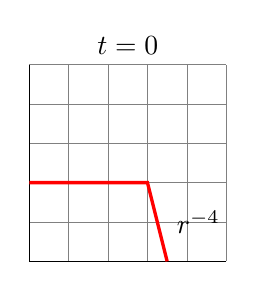
\begin{tikzpicture}
%					Tracé de la grille :
					\draw[step=.5cm,gray,very thin] (0,0) grid (2.5,2.5);
%					Tracé des axes :
					\draw (0,0) -- (0,2.5);
					\draw (0,0) -- (2.5,0);
%					Tracé du graphe :
					\draw[red,very thick] (0,1.0) -- (1.5,1.0) -- (1.75,0);
%					\draw[red,very thick] (1.5,1.0) -- (1.75,0);
					\draw (1.75,0.5) node[right]{$r^{-4}$};
					\draw (1.25,2.5) node[above]{$t = 0$};
				\end{tikzpicture}
			\end{center}
		\end{minipage}\hfill
		\begin{minipage}[b]{0.20\linewidth}
			\begin{center}
				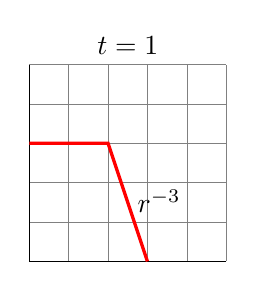
\begin{tikzpicture}
%					Tracé de la grille :
					\draw[step=.5cm,gray,very thin] (0,0) grid (2.5,2.5);
%					Tracé des axes :
					\draw (0,0) -- (0,2.5);
					\draw (0,0) -- (2.5,0);
%					Tracé du graphe :
					\draw[red,very thick] (0,1.5) -- (1,1.5) -- (1.5,0);
%					\draw[red,very thick] (1,1.5) -- (1.5,0);
					\draw (1.25,0.5) node[above right]{$r^{-3}$};
					\draw (1.25,2.5) node[above]{$t = 1$};
				\end{tikzpicture}
			\end{center}
		\end{minipage}\hfill
		\begin{minipage}[b]{0.24\linewidth}
			\begin{center}
				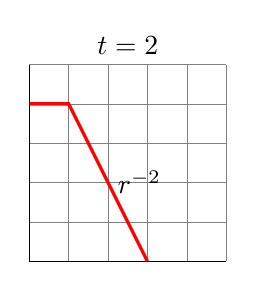
\begin{tikzpicture}
%					Tracé de la grille :
					\draw[step=.5cm,gray,very thin] (0,0) grid (2.5,2.5);
%					Tracé des axes :
					\draw (0,0) -- (0,2.5);
					\draw (0,0) -- (2.5,0);
%					Tracé du graphe :
					\draw[red,very thick] (0,2) -- (0.5,2) -- (1.5,0);
%					\draw[red,very thick] (0.5,2) -- (1.5,0);
					\draw (1,1) node[right]{$r^{-2}$};
					\draw (1.25,2.5) node[above]{$t = 2$};
				\end{tikzpicture}
			\end{center}
		\end{minipage}\hfill
		\begin{minipage}[b]{0.20\linewidth}
			\begin{center}
				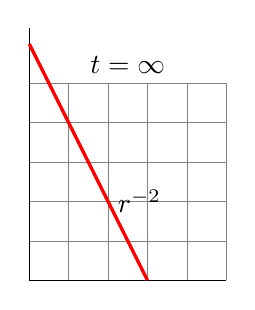
\begin{tikzpicture}
%					Tracé de la grille :
					\draw[step=.5cm,gray,very thin] (0,0) grid (2.5,2.5);
%					Tracé des axes :
					\draw (0,0) -- (0,3.2);
					\draw (0,0) -- (2.5,0);
%					Tracé du graphe :
					\draw[red,very thick] (0,3) -- (1.5,0);
					\draw (1,1) node[right]{$r^{-2}$};
					\draw (1.25,2.5) node[above]{$t = \infty$};
				\end{tikzpicture}
			\end{center}
		\end{minipage}
		\caption{Schéma d'évolution dynamique d'un amas globulaire.\label{schema-effondrement}}
	\end{figure}


%(~la pente $-4$ avec laquelle commence le schéma vient des résultats de simulations numériques~).
%La question à laquelle nous souhaitons répondre est : comment expliquer qu'un amas évolu en augmentant la densité de son cœur et en diminuant la pente avec laquelle le halo décroit ?

%Pour commencer, un amas doit, lorsqu'il est à l'équilibre, suivre un modèle de \textsc{King} ou de sphère isotherme en boîte. Par conséquent, notre amas est au Viriel.
%De plus, le cœur est un systéme auto-gravitant décrit par la thermodynamique. L'un de ses propriétés thermodynamique les plus importante à ce niveau est sa capacité calorifique. En effet :
%Nous cherchons à concentrer la matière dans le cœur de l'amas, et donc y rajouter de la matière à partir du halo (~qui va se diluer~).
%Pour faire diminuer le rayon de l'orbite d'un astre, il faut augmenter sa vitesse~\footnote{rappel : $v^2 = K\left(\frac{2}{r} - \frac{1}{a}\right)$ avec $K = G\left(M+m\right)$
%pour des interactions à deux corps}, et donc sa température. En se rappelant les résultats sur les diagrammes d'énergie de la sphère isotherme, nous nous rendons bien compte que, si la température
%augmente trop, le cœur va passer dans la zone instable, et s'effondrer.

%Le processus pour faire augmenter la température auquel nous nous attèlerons dans la suite est assez simple : l'amas évolue dans le potentiel galactique ; il va en traverser le disque de façon périodique.
%Moments pendant lesquels il va se faire harceler par des forces de marée qui vont lui faire perdre des étoiles. En considérant la description micro canonique, l'énergie est fixé ; or perdre une étoile
%diminue l'énergie potentielle de l'amas. La température va devoir augmenter pour conserver l'énergie totale constante.

%La perte d'étoile apparaît alors comme un processus intéressant pour expliquer l'évolution observée. Les chapitres suivants nous permettront de déterminer, à l'aide de simulation numérique, si la perte
%d'étoile par effet de marée est suffisante pour l'expliquer.





		Pour comprendre ces résultats, il est utile de savoir que plus un amas est âgé
		dynamiquement (plus il est évolué), plus ces temps vont être petits. Ainsi, un amas
		ayant un temps dynamique de $10^{11}$ ans est plus jeune qu'un amas ayant un temps
		dynamique de $10^{8}\ \mathrm{ans}$.

		%: elle passe de très faibles valeurs (entre -10 et -4) pour des amas dynamiquement
		%jeunes, à la valeur caractéristique -2 pour des amas dynamique évolués et
		%correspondant à la pente des coeurs effondrés.
		
		Les graphiques~\ref{Pente-lin_dim} et~\ref{Pente-Td-lin} nous apprennent que
		plus les amas sont âgés, plus la pente de leur halo diminue: elle passe de
		valeurs importantes (entre $-10$ et $-4$) pour des amas dynamiquement jeunes, à la valeur
		$-2$ pour des amas dynamiquement évolués. Notons que cette dernière valeur correspond à la pente des cœurs
		effondrés.
		Le schéma~\ref{schema-effondrement} résume schématiquement cette évolution,
		d'un amas jeune à un amas évolué dont le cœur s'est effondré.

		% Cette évolution est généralement acceptée dans la communauté des spécialiste des amas
		% globulaires. Il n'en demeure pas moins vrai que de nombreux points restent à
		% éclaircir, c'est l'un des objectifs de ce travail.

		Si l'augmentation de la densité centrale au fur et à mesure de l'évolution de l'amas est souvent décrite
		dans la littérature, il n'en est pas de même pour l'évolution de la pente du halo. Nous tenterons de
		préciser ce constat observationnel lors de nos études théoriques et numériques.

		%Cette dernière étude nous montre que plus un amas est âgé, plus la pente de son halo
		%est importante. Dans le chapitre précédent, nous avons relié la pente au paramètre
		%$W_0$ qui, en plus de jouer sur les pentes, joue sur la densité centrale, comme le
		%montre la figure~\ref{King_Modele-test}. Par ailleurs, des simulations partant d'un
		%nuage homogène nous apprennent que la pente du halo après sa formation vaut $-4$. Un
		%amas va donc partir d'une structure cœur-halo avec un cœur de taille importante, un
		%halo de pente $-4$ et va tendre, en vieillissant, vers un amas ayant une densité
		%centrale très élevée dont la pente tend vers $-2$. Puis après un temps infini,
		%l'amas va tendre vers une sphère isotherme. C'est ce que représente le schéma
		%suivant.

		
	\begin{figure}[ht!]
		\begin{minipage}[b]{0.20\linewidth}
			\begin{center}
				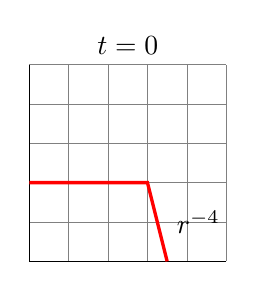
\begin{tikzpicture}
%					Tracé de la grille :
					\draw[step=.5cm,gray,very thin] (0,0) grid (2.5,2.5);
%					Tracé des axes :
					\draw (0,0) -- (0,2.5);
					\draw (0,0) -- (2.5,0);
%					Tracé du graphe :
					\draw[red,very thick] (0,1.0) -- (1.5,1.0) -- (1.75,0);
%					\draw[red,very thick] (1.5,1.0) -- (1.75,0);
					\draw (1.75,0.5) node[right]{$r^{-4}$};
					\draw (1.25,2.5) node[above]{$t = 0$};
				\end{tikzpicture}
			\end{center}
		\end{minipage}\hfill
		\begin{minipage}[b]{0.20\linewidth}
			\begin{center}
				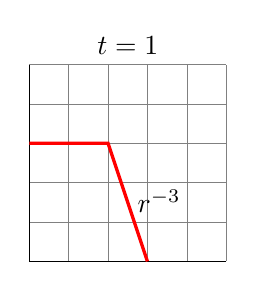
\begin{tikzpicture}
%					Tracé de la grille :
					\draw[step=.5cm,gray,very thin] (0,0) grid (2.5,2.5);
%					Tracé des axes :
					\draw (0,0) -- (0,2.5);
					\draw (0,0) -- (2.5,0);
%					Tracé du graphe :
					\draw[red,very thick] (0,1.5) -- (1,1.5) -- (1.5,0);
%					\draw[red,very thick] (1,1.5) -- (1.5,0);
					\draw (1.25,0.5) node[above right]{$r^{-3}$};
					\draw (1.25,2.5) node[above]{$t = 1$};
				\end{tikzpicture}
			\end{center}
		\end{minipage}\hfill
		\begin{minipage}[b]{0.24\linewidth}
			\begin{center}
				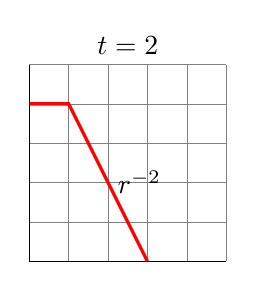
\begin{tikzpicture}
%					Tracé de la grille :
					\draw[step=.5cm,gray,very thin] (0,0) grid (2.5,2.5);
%					Tracé des axes :
					\draw (0,0) -- (0,2.5);
					\draw (0,0) -- (2.5,0);
%					Tracé du graphe :
					\draw[red,very thick] (0,2) -- (0.5,2) -- (1.5,0);
%					\draw[red,very thick] (0.5,2) -- (1.5,0);
					\draw (1,1) node[right]{$r^{-2}$};
					\draw (1.25,2.5) node[above]{$t = 2$};
				\end{tikzpicture}
			\end{center}
		\end{minipage}\hfill
		\begin{minipage}[b]{0.20\linewidth}
			\begin{center}
				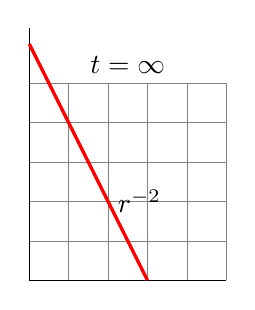
\begin{tikzpicture}
%					Tracé de la grille :
					\draw[step=.5cm,gray,very thin] (0,0) grid (2.5,2.5);
%					Tracé des axes :
					\draw (0,0) -- (0,3.2);
					\draw (0,0) -- (2.5,0);
%					Tracé du graphe :
					\draw[red,very thick] (0,3) -- (1.5,0);
					\draw (1,1) node[right]{$r^{-2}$};
					\draw (1.25,2.5) node[above]{$t = \infty$};
				\end{tikzpicture}
			\end{center}
		\end{minipage}
		\caption{Schéma d'évolution dynamique d'un amas globulaire.\label{schema-effondrement}}
	\end{figure}



		%Pour expliquer cette évolution, nous devons trouver quels phénomènes, de dynamique gravitationnelle, pourraient diluer le halo et concentrer de la matière au centre de l'amas. Le phénomène qui vient le plus naturellement à l'esprit est la perte d'étoiles, pouvant s'effectuer par 2 scénarios :
		%\begin{enumerate}
			%\item des collisions internes qui éjectent des étoiles de l'amas, permettant ainsi au cœur de s'effondrer en essayant de compenser cette perte d'énergie.
			%\item des interactions avec un autre objet massif qui va retirer par effet de marée des étoiles à l'amas, causant l'effondrement de son cœur.
		%\end{enumerate}
		%C'est ce deuxième scénario que nous allons tenter d'étudier.
















%Si la température cinétique du halo augmente, celle du
%cœur va changer pour s'adapter. La capacité calorifique à volume
%constant est négative pour le cœur (~et pour tout système
%auto gravitant~) :
%\begin{align*}
%	E_p &= -2E_c & \text{(~Viriel~)} \\
%	\Rightarrow E &= E_p + E_c = -E_c \\
%	\intertext{or}
%	E_c &\varpropto T \Rightarrow E\varpropto -T \\
%	\intertext{donc}
%	\Rightarrow C_v &= \frac{\partial E}{\partial T} < 0
%\end{align*}
%Cela implique que notre système ne peut que prendre de l'énergie.

%Si la température du cœur augmente, la vitesse de rotation des
%étoiles va augmenter (~$E_c\varpropto T\varpropto v$~), et donc
%leur demi grand axe va diminuer~\footnote{rappel : $v^2 =
%K\left(\frac{2}{r} - \frac{1}{a}\right)$ avec $K = G\left(M+m\right)$
%pour des interactions à deux corps}.
%En conséquent la densité au centre du cœur augmente, augmentant
%ainsi le contraste de densité. Si la température augmente
%suffisamment, le contraste de densité du halo va dépasser la
%valeur critique $\R_c^H$ (~l'énergie est fixé, seul la
%température change, nous utilisons donc la description micro
%canonique~). Le cœur va alors devenir instable.


%	L'interprétation semble simple ici : par exemple : quand les étoiles
%	ont des vitesses de rotation élevées la sphère a une température élevée,
%	et donc sa capacité calorifique à volume constant, $C_v = \frac{\partial H}{\partial T} < 0$
%	(~négatif car $E_p=-2E_c\Rightarrow H=E_c+E_p=-E_c\varpropto-T$~),
%	tend vers $0$ : elle ne peut plus acquérir d'énergie.
%	Si on dépasse la limite de température, elle va devoir se \og~réorganiser~\fg pour
%	rester à l'équilibre et donc pour retourner à un contraste de densité $\R < \R^\beta_c$.
%	Le raisonnement est le même pour la limite en énergie.
		%%Nous avons vu que les courbes~\ref{King_Modele-test} peuvent être divisées en deux parties : l'une, caractérisée par une densité constante, constituant un cœur, et l'autre constituant un halo.
%Nous allons donc considérer un amas d'étoile composé d'un cœur dense et d'un halo.
%Le halo a peu de gravité et se comporte comme un gaz parfait.
%Le comportement observé dans notre étude est résumé sur le schéma~\ref{schema-effondrement} :
%
	\begin{figure}[ht!]
		\begin{minipage}[b]{0.20\linewidth}
			\begin{center}
				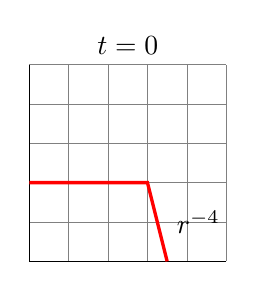
\begin{tikzpicture}
%					Tracé de la grille :
					\draw[step=.5cm,gray,very thin] (0,0) grid (2.5,2.5);
%					Tracé des axes :
					\draw (0,0) -- (0,2.5);
					\draw (0,0) -- (2.5,0);
%					Tracé du graphe :
					\draw[red,very thick] (0,1.0) -- (1.5,1.0) -- (1.75,0);
%					\draw[red,very thick] (1.5,1.0) -- (1.75,0);
					\draw (1.75,0.5) node[right]{$r^{-4}$};
					\draw (1.25,2.5) node[above]{$t = 0$};
				\end{tikzpicture}
			\end{center}
		\end{minipage}\hfill
		\begin{minipage}[b]{0.20\linewidth}
			\begin{center}
				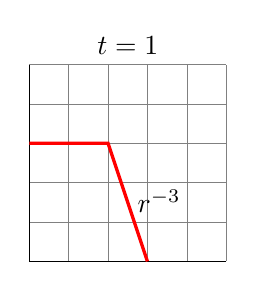
\begin{tikzpicture}
%					Tracé de la grille :
					\draw[step=.5cm,gray,very thin] (0,0) grid (2.5,2.5);
%					Tracé des axes :
					\draw (0,0) -- (0,2.5);
					\draw (0,0) -- (2.5,0);
%					Tracé du graphe :
					\draw[red,very thick] (0,1.5) -- (1,1.5) -- (1.5,0);
%					\draw[red,very thick] (1,1.5) -- (1.5,0);
					\draw (1.25,0.5) node[above right]{$r^{-3}$};
					\draw (1.25,2.5) node[above]{$t = 1$};
				\end{tikzpicture}
			\end{center}
		\end{minipage}\hfill
		\begin{minipage}[b]{0.24\linewidth}
			\begin{center}
				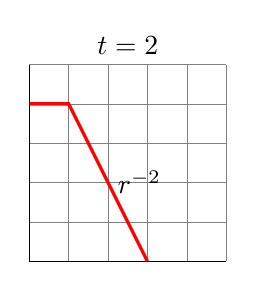
\begin{tikzpicture}
%					Tracé de la grille :
					\draw[step=.5cm,gray,very thin] (0,0) grid (2.5,2.5);
%					Tracé des axes :
					\draw (0,0) -- (0,2.5);
					\draw (0,0) -- (2.5,0);
%					Tracé du graphe :
					\draw[red,very thick] (0,2) -- (0.5,2) -- (1.5,0);
%					\draw[red,very thick] (0.5,2) -- (1.5,0);
					\draw (1,1) node[right]{$r^{-2}$};
					\draw (1.25,2.5) node[above]{$t = 2$};
				\end{tikzpicture}
			\end{center}
		\end{minipage}\hfill
		\begin{minipage}[b]{0.20\linewidth}
			\begin{center}
				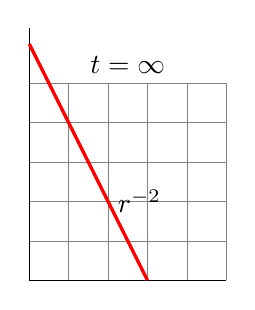
\begin{tikzpicture}
%					Tracé de la grille :
					\draw[step=.5cm,gray,very thin] (0,0) grid (2.5,2.5);
%					Tracé des axes :
					\draw (0,0) -- (0,3.2);
					\draw (0,0) -- (2.5,0);
%					Tracé du graphe :
					\draw[red,very thick] (0,3) -- (1.5,0);
					\draw (1,1) node[right]{$r^{-2}$};
					\draw (1.25,2.5) node[above]{$t = \infty$};
				\end{tikzpicture}
			\end{center}
		\end{minipage}
		\caption{Schéma d'évolution dynamique d'un amas globulaire.\label{schema-effondrement}}
	\end{figure}


%(~la pente $-4$ avec laquelle commence le schéma vient des résultats de simulations numériques~).
%La question à laquelle nous souhaitons répondre est : comment expliquer qu'un amas évolu en augmentant la densité de son cœur et en diminuant la pente avec laquelle le halo décroit ?

%Pour commencer, un amas doit, lorsqu'il est à l'équilibre, suivre un modèle de \textsc{King} ou de sphère isotherme en boîte. Par conséquent, notre amas est au Viriel.
%De plus, le cœur est un systéme auto-gravitant décrit par la thermodynamique. L'un de ses propriétés thermodynamique les plus importante à ce niveau est sa capacité calorifique. En effet :
%Nous cherchons à concentrer la matière dans le cœur de l'amas, et donc y rajouter de la matière à partir du halo (~qui va se diluer~).
%Pour faire diminuer le rayon de l'orbite d'un astre, il faut augmenter sa vitesse~\footnote{rappel : $v^2 = K\left(\frac{2}{r} - \frac{1}{a}\right)$ avec $K = G\left(M+m\right)$
%pour des interactions à deux corps}, et donc sa température. En se rappelant les résultats sur les diagrammes d'énergie de la sphère isotherme, nous nous rendons bien compte que, si la température
%augmente trop, le cœur va passer dans la zone instable, et s'effondrer.

%Le processus pour faire augmenter la température auquel nous nous attèlerons dans la suite est assez simple : l'amas évolue dans le potentiel galactique ; il va en traverser le disque de façon périodique.
%Moments pendant lesquels il va se faire harceler par des forces de marée qui vont lui faire perdre des étoiles. En considérant la description micro canonique, l'énergie est fixé ; or perdre une étoile
%diminue l'énergie potentielle de l'amas. La température va devoir augmenter pour conserver l'énergie totale constante.

%La perte d'étoile apparaît alors comme un processus intéressant pour expliquer l'évolution observée. Les chapitres suivants nous permettront de déterminer, à l'aide de simulation numérique, si la perte
%d'étoile par effet de marée est suffisante pour l'expliquer.








Cette dernière étude nous montre que plus un amas est âgé, plus la pente de son halo est importante.
Dans le chapitre précédent, nous avons relié la pente au paramètre $W_0$ qui, en plus de jouer sur les pentes, joue sur la densité centrale, comme le montre la figure~\ref{King_Modele-test}.
Par ailleurs, des simulations partant d'un nuage homogène nous apprennent que la pente du halo après sa formation vaut $-4$.
Un amas va donc partir d'une structure cœur-halo avec un cœur de taille importante, un halo de pente $-4$ et va tendre, en vieillissant, vers un amas ayant une densité centrale très élevée dont la pente tend vers $-2$.
Puis après un temps infini, l'amas va tendre vers une sphère isotherme.
C'est ce que représente le schéma suivant.


	\begin{figure}[ht!]
		\begin{minipage}[b]{0.20\linewidth}
			\begin{center}
				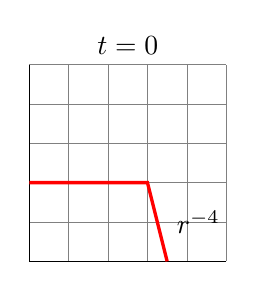
\begin{tikzpicture}
%					Tracé de la grille :
					\draw[step=.5cm,gray,very thin] (0,0) grid (2.5,2.5);
%					Tracé des axes :
					\draw (0,0) -- (0,2.5);
					\draw (0,0) -- (2.5,0);
%					Tracé du graphe :
					\draw[red,very thick] (0,1.0) -- (1.5,1.0) -- (1.75,0);
%					\draw[red,very thick] (1.5,1.0) -- (1.75,0);
					\draw (1.75,0.5) node[right]{$r^{-4}$};
					\draw (1.25,2.5) node[above]{$t = 0$};
				\end{tikzpicture}
			\end{center}
		\end{minipage}\hfill
		\begin{minipage}[b]{0.20\linewidth}
			\begin{center}
				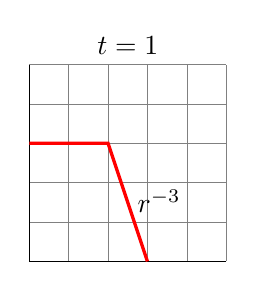
\begin{tikzpicture}
%					Tracé de la grille :
					\draw[step=.5cm,gray,very thin] (0,0) grid (2.5,2.5);
%					Tracé des axes :
					\draw (0,0) -- (0,2.5);
					\draw (0,0) -- (2.5,0);
%					Tracé du graphe :
					\draw[red,very thick] (0,1.5) -- (1,1.5) -- (1.5,0);
%					\draw[red,very thick] (1,1.5) -- (1.5,0);
					\draw (1.25,0.5) node[above right]{$r^{-3}$};
					\draw (1.25,2.5) node[above]{$t = 1$};
				\end{tikzpicture}
			\end{center}
		\end{minipage}\hfill
		\begin{minipage}[b]{0.24\linewidth}
			\begin{center}
				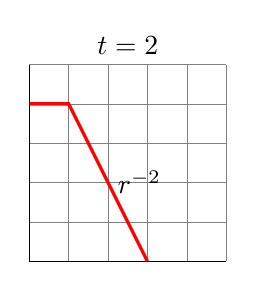
\begin{tikzpicture}
%					Tracé de la grille :
					\draw[step=.5cm,gray,very thin] (0,0) grid (2.5,2.5);
%					Tracé des axes :
					\draw (0,0) -- (0,2.5);
					\draw (0,0) -- (2.5,0);
%					Tracé du graphe :
					\draw[red,very thick] (0,2) -- (0.5,2) -- (1.5,0);
%					\draw[red,very thick] (0.5,2) -- (1.5,0);
					\draw (1,1) node[right]{$r^{-2}$};
					\draw (1.25,2.5) node[above]{$t = 2$};
				\end{tikzpicture}
			\end{center}
		\end{minipage}\hfill
		\begin{minipage}[b]{0.20\linewidth}
			\begin{center}
				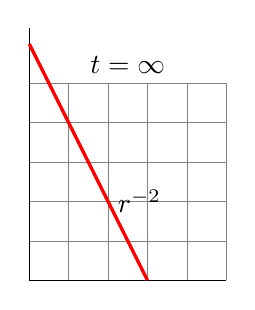
\begin{tikzpicture}
%					Tracé de la grille :
					\draw[step=.5cm,gray,very thin] (0,0) grid (2.5,2.5);
%					Tracé des axes :
					\draw (0,0) -- (0,3.2);
					\draw (0,0) -- (2.5,0);
%					Tracé du graphe :
					\draw[red,very thick] (0,3) -- (1.5,0);
					\draw (1,1) node[right]{$r^{-2}$};
					\draw (1.25,2.5) node[above]{$t = \infty$};
				\end{tikzpicture}
			\end{center}
		\end{minipage}
		\caption{Schéma d'évolution dynamique d'un amas globulaire.\label{schema-effondrement}}
	\end{figure}



Pour expliquer cette évolution, nous devons trouver quels phénomènes, de dynamique gravitationnelle, pourraient diluer le halo et concentrer de la matière au centre de l'amas. Le phénomène qui vient le plus naturellement à l'esprit est la perte d'étoiles, pouvant s'effectuer par 2 scénarios :
\begin{enumerate}
	\item des collisions internes qui éjectent des étoiles de l'amas, permettant ainsi au cœur de s'effondrer en essayant de compenser cette perte d'énergie.
	\item des interactions avec un autre objet massif qui va retirer par effet de marée des étoiles à l'amas, causant l'effondrement de son cœur.
\end{enumerate}
C'est ce deuxième scénario que nous allons tenter d'étudier.
















%Si la température cinétique du halo augmente, celle du
%cœur va changer pour s'adapter. La capacité calorifique à volume
%constant est négative pour le cœur (~et pour tout système
%auto gravitant~) :
%\begin{align*}
%	E_p &= -2E_c & \text{(~Viriel~)} \\
%	\Rightarrow E &= E_p + E_c = -E_c \\
%	\intertext{or}
%	E_c &\varpropto T \Rightarrow E\varpropto -T \\
%	\intertext{donc}
%	\Rightarrow C_v &= \frac{\partial E}{\partial T} < 0
%\end{align*}
%Cela implique que notre système ne peut que prendre de l'énergie.

%Si la température du cœur augmente, la vitesse de rotation des
%étoiles va augmenter (~$E_c\varpropto T\varpropto v$~), et donc
%leur demi grand axe va diminuer~\footnote{rappel : $v^2 =
%K\left(\frac{2}{r} - \frac{1}{a}\right)$ avec $K = G\left(M+m\right)$
%pour des interactions à deux corps}.
%En conséquent la densité au centre du cœur augmente, augmentant
%ainsi le contraste de densité. Si la température augmente
%suffisamment, le contraste de densité du halo va dépasser la
%valeur critique $\R_c^H$ (~l'énergie est fixé, seul la
%température change, nous utilisons donc la description micro
%canonique~). Le cœur va alors devenir instable.


%	L'interprétation semble simple ici : par exemple : quand les étoiles
%	ont des vitesses de rotation élevées la sphère a une température élevée,
%	et donc sa capacité calorifique à volume constant, $C_v = \frac{\partial H}{\partial T} < 0$
%	(~négatif car $E_p=-2E_c\Rightarrow H=E_c+E_p=-E_c\varpropto-T$~),
%	tend vers $0$ : elle ne peut plus acquérir d'énergie.
%	Si on dépasse la limite de température, elle va devoir se \og~réorganiser~\fg pour
%	rester à l'équilibre et donc pour retourner à un contraste de densité $\R < \R^\beta_c$.
%	Le raisonnement est le même pour la limite en énergie.


	\section{Les Galaxies}%{Que peut-on dire des autres ...!}
		En reprenant l'introduction de~\cite{binntre},
		nous pouvons proposer la définition suivante d'une galaxie:
		\begin{quote}
			Une galaxie est un objet composé de $10^5$ à plusieurs milliards d'étoiles, liées gravitationnellement, de gaz et dont la masse
			est supérieure à $10^7M_\odot$.
		\end{quote}

		\subsection{Historique}

			L'observation des galaxies a commencé avec Charles Messier, qui les
			catalogua alors qu'il recherchait des comètes pour éviter de passer
			inutilement du temps sur ces objets \og nébuleux\fg{}.

			Depuis, les techniques d'observation ont évolué, les astronomes ont
			commencé à pouvoir distinguer de plus en plus de détails, et ont pu
			mesurer leurs profils de luminosité. Ces objets \og{}nébuleux\fg ont été classés dans
			plusieurs catégories:
			\begin{itemize}
				\item les nébuleuses, composées de gaz et peut-être d'étoiles en formation;
				\item les amas globulaires;
				\item les galaxies.
			\end{itemize}
			Une autre catégorie d'objet est apparue plus tardivement: les groupes de galaxies.

			Au début des années 1930, Zwicky, travaillant sur l'amas de galaxies Coma, se rendit compte que la masse
			gravitationnelle ne correspondait pas à la masse lumineuse (voir~\cite{1933AcHPh...6..110Z}): si l'on suppose, comme le fait
			Zwicky, que l'amas de la Coma est dans un état d'équilibre, le théorème du viriel impose alors que sa masse, son rayon
			$R$ et la vitesse caractéristique de ses composantes vérifient la relation $GM = R v^{1/2}$. À l'époque, un facteur 100
			apparaissait entre la masse visible (obtenue en sommant la masse de chaque galaxie de l'amas) et la masse nécessaire pour être
			au viriel. Malgré la précision plus importante des données d'aujourd'hui, et la meilleure prise en compte des différentes
			composantes (gaz, étoiles...), le problème persiste toujours et a permis l'introduction de la matière noire. Quelques années
			plus tard, \cite{1939LicOB..19...41B} pointa que la courbe de rotation des galaxies elle-même nécessitait également
			l'introduction de matière noire.
			% Un autre problème observationnel ayant besoin de matière noire: la courbe de rotation des galaxies
			% (voir~\cite{1939LicOB..19...41B}): passé un certain rayon, la vitesse de rotation des étoiles dans la galaxie devient
			% constante~! Là aussi, il a fallu ajouter de la matière invisible.

			% Au début des années 30, \bsc{Zwicky}, travaillant sur le groupe de galaxies \bsc{Coma}, se rendit compte que la masse
			% gravitationnelle et la masse lumineuse (le ratio masse-luminosité) ne correspondait pas: il y a de la masse invisible. La
			% confirmation suivante arriva lors de l'observation des courbes de vitesse de rotation des galaxies, au début des années 1970
			% par Vera Rubin. Ces courbes présentait un plateau qui n'était explicable par la théorie que en ajoutant une nouvelle
			% composante de matière: la matière noire.

			Depuis lors, nombre de travaux ont été menés, à la fois sur les halos de
			matière noire et sur les profils de luminosité (et donc de densité de masse)
			des galaxies.

		\subsection{Les différents types de galaxies}

			Les galaxies naines sphéroïdales, ou galaxies à faible brillance de surface (LSB), sont des
			galaxies très difficile à observer. Elles ne le sont actuellement que dans notre groupe local,
			où elles sont les plus nombreuses (d'après \citet{2013MNRAS.429.3068T}). Ce sont des galaxies
			avec peu de gaz et un grand rapport masse/luminosité, ce dernier point laissant entendre qu'elles
			sont dominées par la matière noire. \cite{2001ApJ...552L..23D} ont étudié le profil
			de densité d'une cinquantaine de ces LSB et remarqué qu'elles avaient toutes un profil cœur-halo.

			Les galaxies spirales ont une structure plus compliquée, dont la partie visible, détaillée sur la
			figure~\ref{Fig::Intro::schemaGS}, se décompose  habituellement de la façon suivante:
			\begin{itemize}
				\item le bulbe, pouvant abriter un trou noir super-massif;
				\item le disque, composé lui-même de deux parties: le disque épais
					et le disque mince;
				\item le halo stellaire, dans lequel évoluent notamment les amas globulaires.
			\end{itemize}
			Un halo de matière noire sphéroïdal (non représenté sur la figure~\ref{Fig::Intro::schemaGS}) englobe le tout.

			\begin{figure}[h]
				\begin{center}
					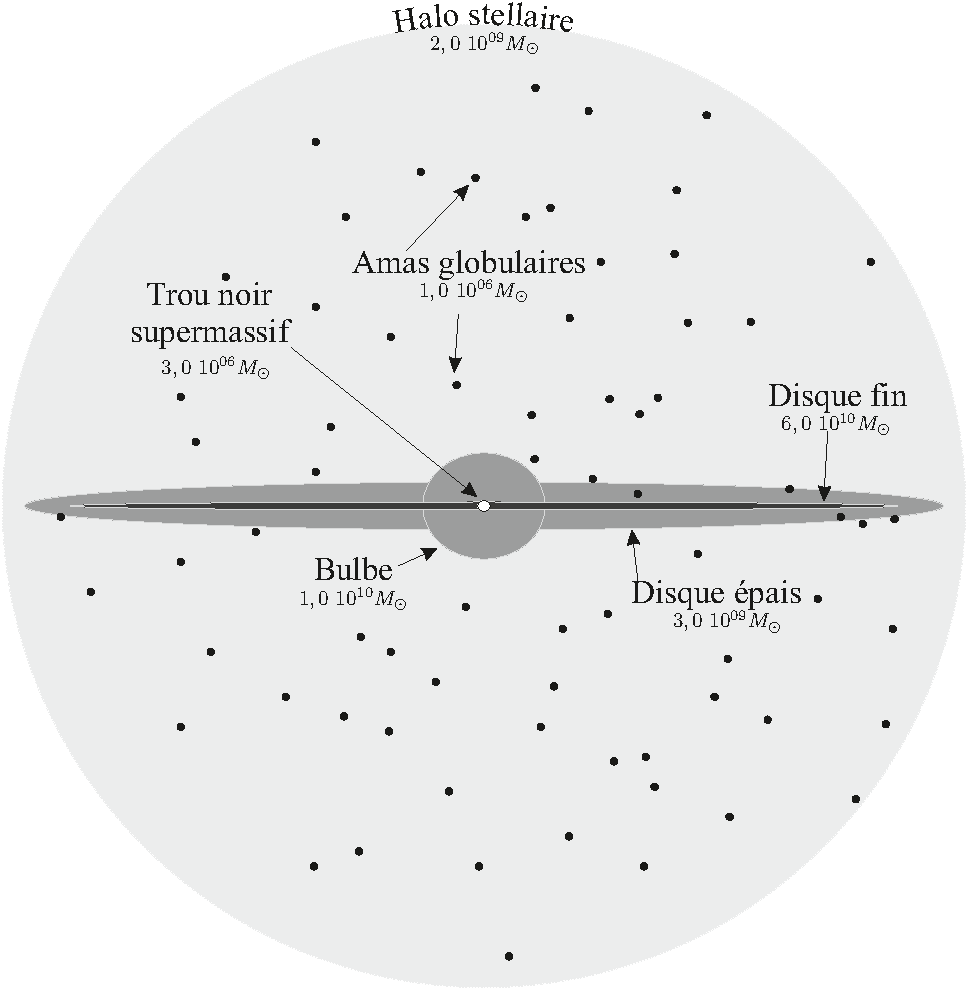
\includegraphics[scale=0.5]{voielactee}
				\end{center}
				\caption{Structure visible d'une galaxie spirale (figure extraite de~\citet{CoursJP}).\label{Fig::Intro::schemaGS}}
			\end{figure}

			% Et enfin les galaxies elliptiques qui sont généralement les
			La dernière classe principale est celle des galaxies elliptiques. Ces galaxies sont essentiellement
			constituées d'étoiles vieilles et ne contiennent que très
			peu de gaz.

		\subsection{Profils de matière noire}

			% Merrit et al
			\cite{2006AJ....132.2685M,2006AJ....132.2701G,2006AJ....132.2711G}
			ont menés une étude exhaustive des profils de matière
			noire dont la distribution a pu être mise en évidence
			autour des galaxies et dans les simulations numériques.

			Il ressort de cette étude qu'il n'existe pas réellement de profil universel, contrairement à ce qu'il fut suggéré par les travaux de la fin du \romannumeral 20
			\textsuperscript{e}~siècle (voir par exemple~\cite{NFW+97}), même si le concept de profil universel reste une bonne première approximation. Chaque halo de matière noire pour chaque
			type de galaxie doit être ajusté par un profil différent. Comme nous l'avons vu plus haut, les galaxies naines ont un profil
			de type cœur-halo, et ce sont les seules à posséder un cœur. Les galaxies spirales et elliptiques possèdent généralement un profil
			montrant un cusp à la place du cœur (un profil de type cuspide) ajusté correctement par un profil de Vaucouleurs.
			% correctement par un profil dit de Dehnen-McLaughin. Ce profil est directement issu d'une généralisation du profil de
			% Vaucouleurs: le profil de Einasto $R^{1/N}$.

			%ont une préférence pour les profil cupsy de Prugniel \&
			%Simien ou encore Dehnen-McLaughlin.

			Dès 1948, Gérard de Vaucouleurs remarqua que de nombreuses galaxies elliptiques possédaient une
			brillance de surface projetée variant comme:
			\begin{align}
				I(R) = I_\mathrm{eff} 10^{-3.3307\left[\(\dfrac{R}{R_\mathrm{eff}}\)^{1/4} - 1\right]}
			\end{align}
			avec $R$ le rayon projeté.
			C'est la fameuse loi de de Vaucouleurs. Depuis de nombreux modèles ont étendu celle-ci:
			\begin{itemize}
				\item le modèle empirique d'Einasto~\footnote{Ce modèle est bel et bien empirique car il est obtenu directement en
					remplaçant la brillance par la densité sans aucun calcul.} qui propose une densité volumique de masse de la
					forme:
					\begin{align}
						\rho(r) = \rho_e \exp\left[-d_n\left\{\(\dfrac{r}{r_e}\)^{1/n} - 1\right\}\right] \label{Intro::Eq::Einasto}
					\end{align}
					avec $\rho_e = \rho(r_e)$ et $r_e$ le rayon à 50\% de masse;
				\item le modèle de Prugniel-Simien, moins empirique que le précédent, est obtenu en déprojetant partiellement la loi de de
					Vaucouleurs, la densité est de la forme:
					\begin{align}
						\rho(r) = \rho_0\(\dfrac{r}{R_e}\)^{-p_n}\exp\left[-b_n\left\{\(\dfrac{r}{R_e}\)^{1/n}-1\right\}\right].\label{Intro::Eq::P-S}
					\end{align}
			\end{itemize}

			% Les profils des structures formées à l'échelle
			Les profils des halos de matière noire formés à l'échelle
			galactique dans les simulations numériques sont quelque
			peu différents. En première approximation, le modèle
			NFW, couramment utilisé, convient. Mais les études plus
			fines menées par \cite{2006AJ....132.2685M,2006AJ....132.2701G,2006AJ....132.2711G} montrent que
			les profils de de Vaucouleurs généralisé~\ref{Intro::Eq::Einasto} et~\ref{Intro::Eq::P-S} conviennent mieux.
			% Einasto (issu d'une déprojection d'une brillance de
			% surface projetée en $R^{1/N}$) convient mieux. Ce
			% profil est issu de la même famille que les modèle de
			% Prugniel-Simien et Dehnen-McLaughin.

			%Pour les simulations numériques, c'est un peu
			%différent; de par sa simplicité les gens préfère
			%utiliser le profil de Navarro-Frenk-White, NFW. Or, et
			%cela est démontré dans la série d'article, le meilleur
			%profil pour les halos de matière noire est le Einasto
			%$R^{1/N}$.

		\subsection{Scénario de formation}
			Le scénario de formation des galaxies le plus généralement admis aujourd'hui est le scénario
			hiérarchique. Dans ce scénario, les plus petites structures, comme les galaxies naines, ont
			été les premières à se former. Puis, au fil des interactions, elles fusionnent pour former
			des structures de plus en plus grosses. Ainsi arrivent les galaxies spirales, puis
			elliptiques.

			% Cependant, ce modèle apporte son lot de problème. Notamment, il prévoit que les halos de matière
			% noire soit des cupsides là où les observations trouvent des cœur-halo, ou encore la quantité de
			% petite structure, tel les amas globulaire et les LSB, qui devrait être beaucoup plus importante autour de
			% notre galaxie.

			Cependant, ce modèle apporte son lot de problèmes:
			\begin{itemize}
				\item les simulations mettant en jeu ce processus montrent des profils de type cuspide pour les halos de matière noire
					% il prévoit une structure de type cupside pour les halos de matière noire
					alors que les observations montrent que les galaxies naines possèdent un cœur et un halo et qu'elles sont très
					nombreuses;
				\item dans les modèles numériques de formation hiérarchique, le nombre de petites
					structures (amas globulaire et LSB) est beaucoup plus important que dans les
					observations (voir \citet{2006CombesBook} et les nombreuses références contenues dans ce livre).
				% \item la quantité de petite structure, tel les amas globulaire et les LSB, qui devrait
					% être beaucoup plus importante autour de notre galaxie.
			\end{itemize}

			Ces problèmes sont observés dans les simulations de formation de grande structures. Très peu d'études théoriques peuvent être
			menées sur ces échelles spatiales et temporelles. Nous pouvons cependant envisager certaines situations théoriques dans
			lesquelles certains aspects de ces problèmes peuvent être étudiés. C'est l'objet de la prochaine partie.
